% !TEX encoding = UTF-8 Unicode
\documentclass{article}
%\documentclass[12pt,reqno]{amsart}
\usepackage[russian]{babel}
\usepackage[utf8]{inputenc}
%\usepackage[dvips]{graphicx,graphics}
\usepackage{graphicx}
\usepackage{euscript}
\usepackage{graphics}
%\usepackage{russcorr}
\usepackage[active]{srcltx} % SRC Specials: DVI [Inverse] Search
\usepackage{amssymb,amsmath,amsthm,amsfonts}
\usepackage{amsopn}
\newtheorem{cor}{Следствие}
\newtheorem{lem}{Лемма}
\newtheorem{thm}{Теорема}
\newtheorem{prop}{Предложение}
\newtheorem*{thm_pres}{Теорема}
\theoremstyle{definition}
\newtheorem{defn}{Определение}
\newtheorem{defneq}{Эквивалентное определение}
\theoremstyle{remark}
\newtheorem*{rem}{Замечание}
\newtheorem*{deff}{Обозначение}
\usepackage{verbatim}
\usepackage{listings}
\usepackage{hyperref}
\usepackage{color}

\definecolor{dkgreen}{rgb}{0,0.5,0}
\definecolor{gray}{rgb}{0.5,0.5,0.5}
\definecolor{mauve}{rgb}{0.58,0,0.52}

\lstset{frame=tb,
  language=Java,
  aboveskip=3mm,
  belowskip=3mm,
  showstringspaces=false,
  columns=flexible,
  basicstyle={\small\ttfamily},
  numbers=none,
  numberstyle=\tiny\color{gray},
  keywordstyle=\color{blue},
  commentstyle=\color{dkgreen},
  stringstyle=\color{mauve},
  breaklines=true,
  breakatwhitespace=true,
  tabsize=3
}

\newcommand{\sug}[1]{\rule[-2mm]{0.4pt}{5mm}_{\,{#1}}}
\newcommand{\gen} {$GE^+_n(\mathbf{R}[x])\ $}
\newcommand{\genn} {$GE^+_2(\mathbf{R}[x])\ $}
\newcommand{\gn} {$G_n(\mathbf{R})\ $}
\newcommand{\gln} {$GL_n(\mathbf{R}[x])\ $}
\newcommand{\p} {\mathbf{P}}
\newcommand{\peq} {$\mathcal{P}$}
\newcommand{\po} {$\mathcal{P}_0$}
\newcommand{\ff} {$\mathbf{R}\ $}
\newcommand{\fx} {\mathbf{R}[x]}
\newcommand{\fp} {\mathbf{R_+}}
\newcommand{\fxp} {\mathbf{R_+}[x]}
\newcommand{\zx} {\mathbb{Z}[x]}
\newcommand{\zxp} {\mathbb{Z_+}[x]}
\newcommand{\basering} {$\mathbf{F}$}
\newcommand{\lfrac} [2] {\displaystyle \frac{#1}{#2}}
\newcommand{\brsum} [3] {\displaystyle \sum \limits_{#1}^{#2} \left( #3\right)}
\newcommand{\lsum} [2] {\displaystyle \sum \limits_{#1}^{#2}}
\newcommand{\br} [1] {\left( #1 \right)}
\newcommand{\tab} {\mbox{             } \quad }
\usepackage{a4wide}

\usepackage{verbatim}
\usepackage{hyperref}
\hypersetup{
    colorlinks,
    citecolor=black,
    filecolor=black,
    linkcolor=blue,
    urlcolor=blue
}
\setcounter{secnumdepth}{0}


\begin{document}
\section*{Отчет по первому практическому заданию}
\section*{Царькова Анастасия}

Формулы для градиента и гессиана функции логистической регрессии:

$$
f(x) = \lfrac{1}{m} \sum_{i = 1}^m \ln(1 + \exp(-b_ia_i^Tx)) + \lfrac{\lambda}{2} \|x\|_2^2 = \lfrac{1}{m} \ln(1 + \exp(-b * Ax)) + \lfrac{\lambda}{2} x^Tx
$$

$$
\nabla f(x) = -\lfrac{1}{m} A^T \left(b * \left(\lfrac{1}{1 - \exp(b * Ax)} \right)\right) + \lambda x = -\lfrac{1}{m} A^T \left(b * Expit(-b * Ax)\right) + \lambda x
$$

$$
\nabla^2 f(x) = \lfrac{1}{m} A^T Diag\left(\left(1 - \left(\lfrac{1}{1 - \exp(b * Ax)} \right)\right) * \left(\lfrac{1}{1 - \exp(b * Ax)} \right)\right)A + \lambda I =
$$

$$
= \lfrac{1}{m} A^T Diag\left(1 - Expit(b * Ax)\right) * \left(Expit(-b * Ax)\right)A + \lambda I
$$


(Далее все комментарии к графикам над ними>)

\section{Зависимость поведения метода от обусловленности функции.}


В данном эксперименте предлагается проанализировать траекторию градиентного спуска в зависимости от:

1. Обусловленности функции

2. Выбора начальной точки

3. Стратегии выбора шага



Сравнивая графики с линиями уровня функции и траекториями методов.



Зададим объекты на которых будем сравнивать поведения методов:

1. Функции --  двумерные квадратичные функции с d равным нулю(для простоты) $f(x) = x^TAx + bx = x^TAx$.

$$
M_1 =
\begin{pmatrix}
1 &	0\\
0 &	2
\end{pmatrix}\ M_2 =
\begin{pmatrix}
1 &	0\\
0 &	60
\end{pmatrix}
$$


2. Начальные точки

$$
x_1 =
\begin{pmatrix}
1 \\
1
\end{pmatrix}\ x_2 =
\begin{pmatrix}
20 \\
30
\end{pmatrix}
$$

3. Cтратегии выбора шага: Armijo, Wolfe, Constant\\


Результаты эксперимента:\\


$\bullet$ Constant\\

Видно что метод работает не очень хорошо. Делает слишком много шагов, но не слишком чувствителен к выбору начальной точки.

Более того крайне чувствителен к обусловленности функции, на $M_2$ метод возвращает $computational\_error$, поэтому я взяла вместо нее
$
M =\begin{pmatrix}1 &	0\\ 0 &	10
\end{pmatrix}
$
и все равно получила $iterations\_exceeded$, но полученные графики очень показательны. Кажется что метод вряд ли сойдется при увеличении числа итераций.

Данный метод очевидно является плохим, потому что если выбрать "плохой" шаг то можно не сойтись никогда.
\begin{center}
\begin{tabular}{cc}
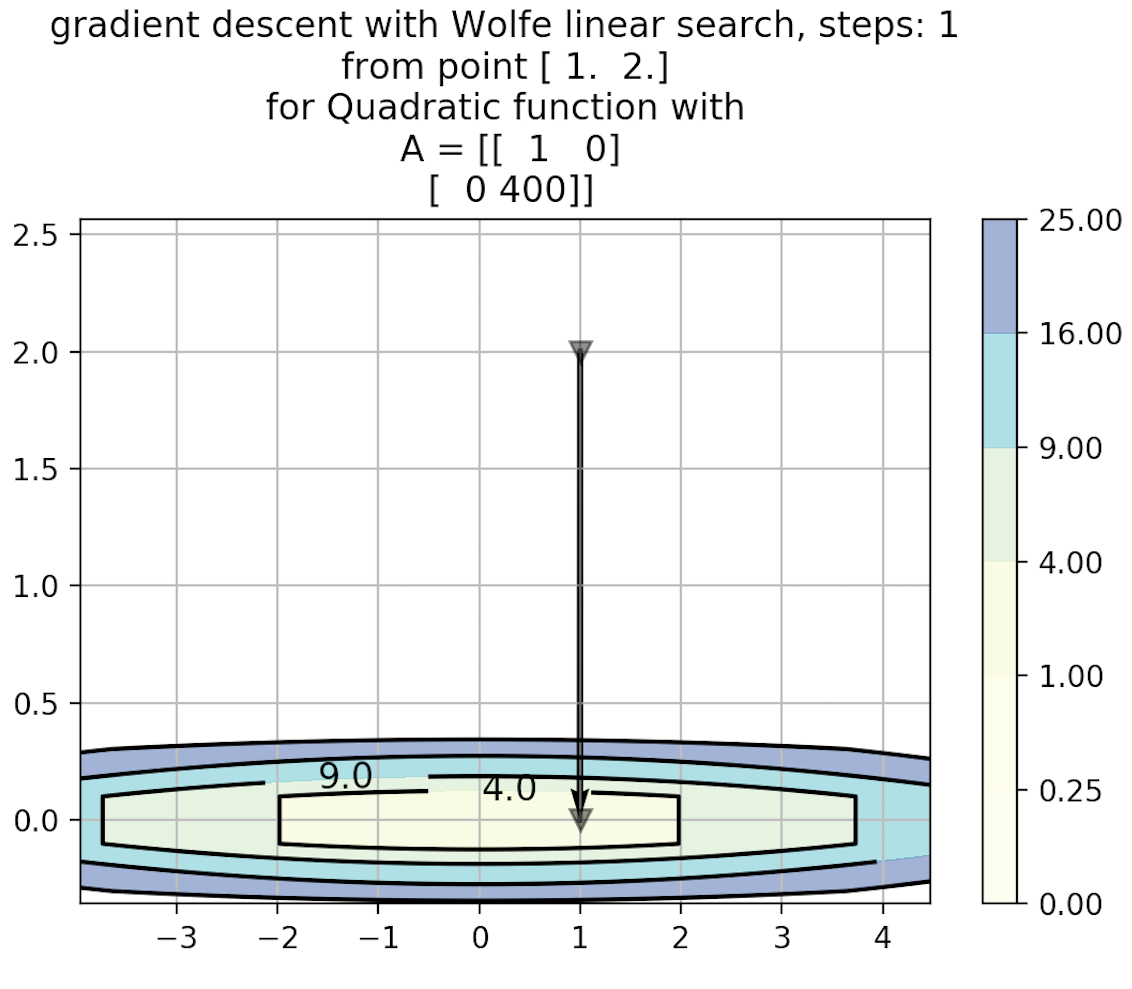
\includegraphics[width=0.49\linewidth]{15.png} &
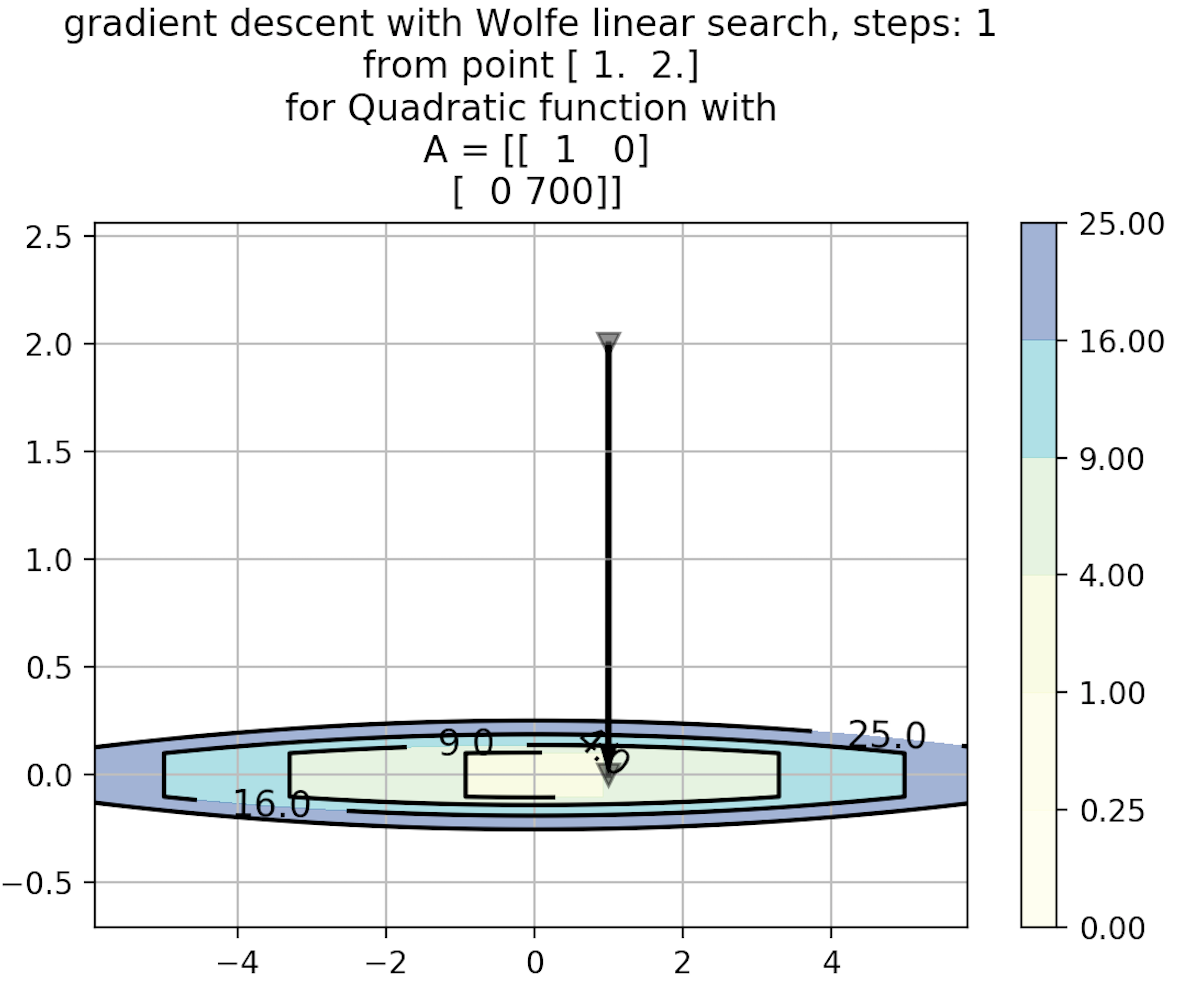
\includegraphics[width=0.49\linewidth]{16.png} \\
 a)$M_1,\ x_1$ & b)$M_1,\ x_2$\\
\end{tabular}
\end{center}
\begin{center}
\begin{tabular}{cc}
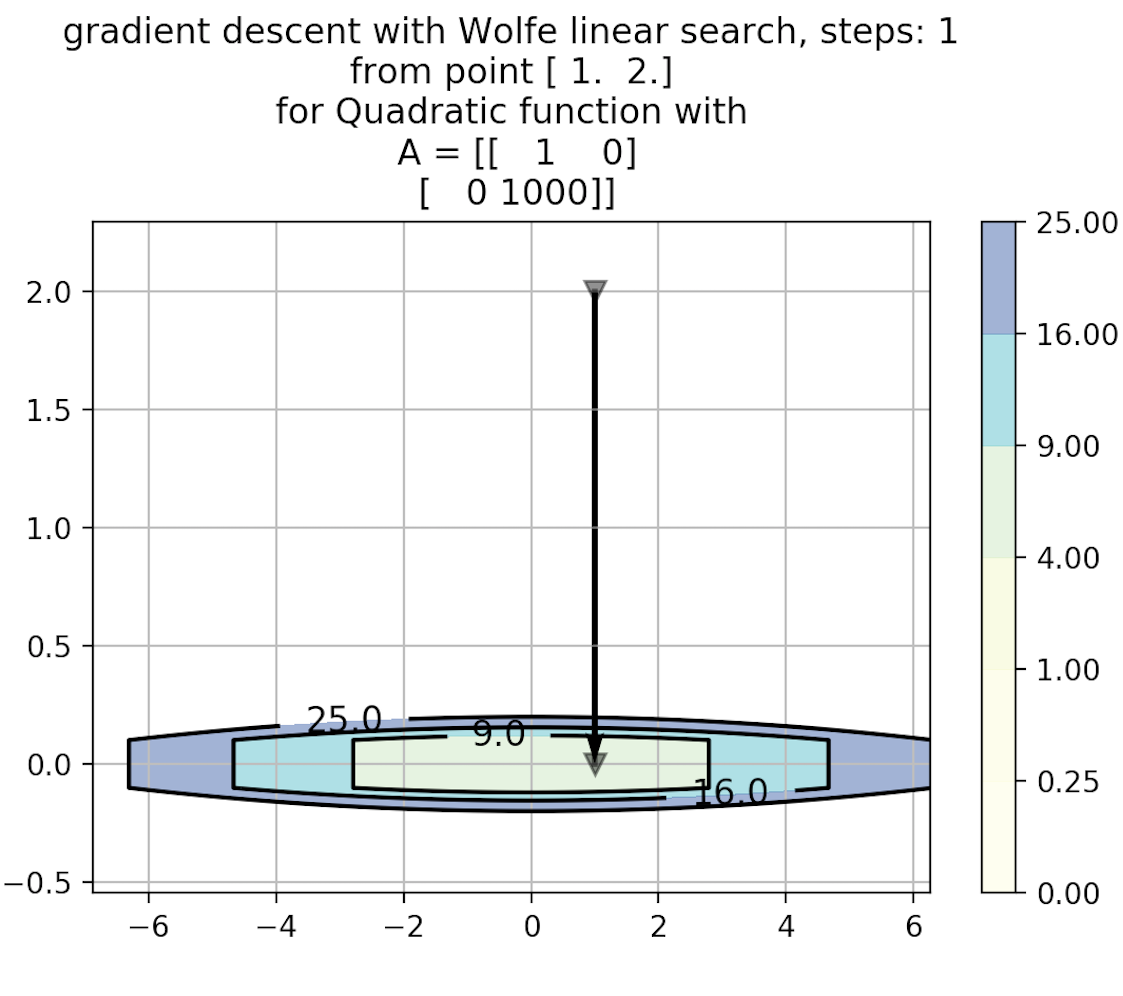
\includegraphics[width=0.49\linewidth]{17.png} &
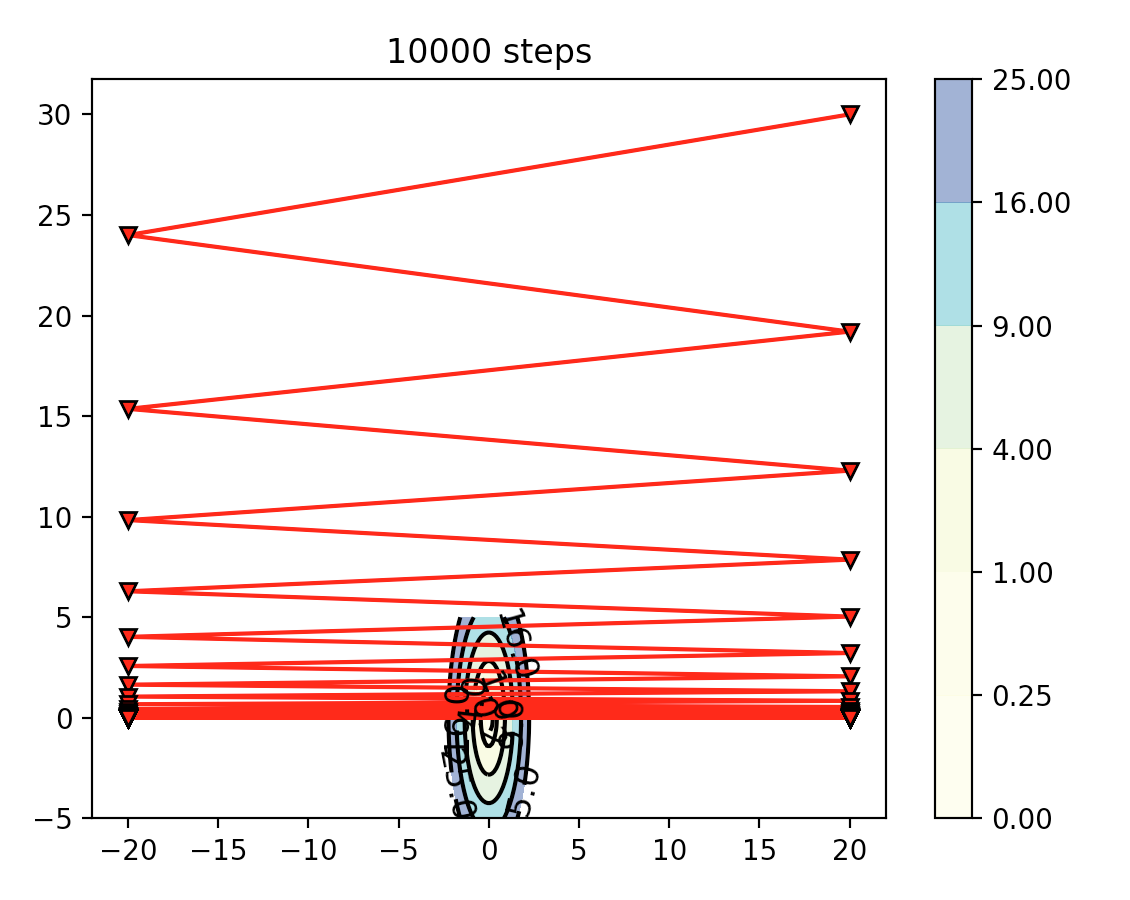
\includegraphics[width=0.49\linewidth]{18.png} \\
 a)$M,\ x_1$ & b)$M,\ x_2$\\
\end{tabular}
\end{center}

$\bullet$ Armijo

Данные метод явно лучше предыдущего.
Видно что метод очень чувствителен к обусловленности функции. Так же есть небольшая зависимость о выбора начальной точки.

\begin{center}
\begin{tabular}{cc}
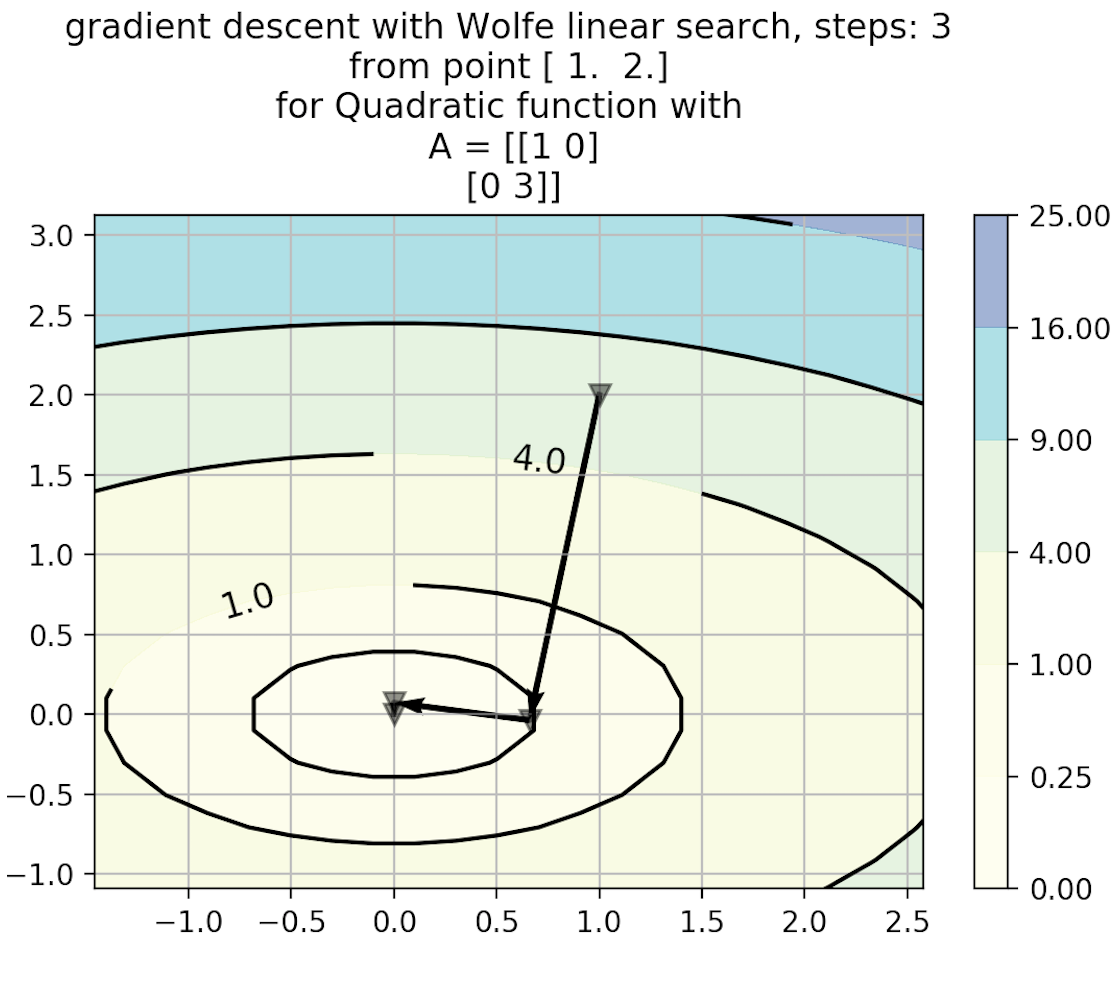
\includegraphics[width=0.49\linewidth]{11.png} &
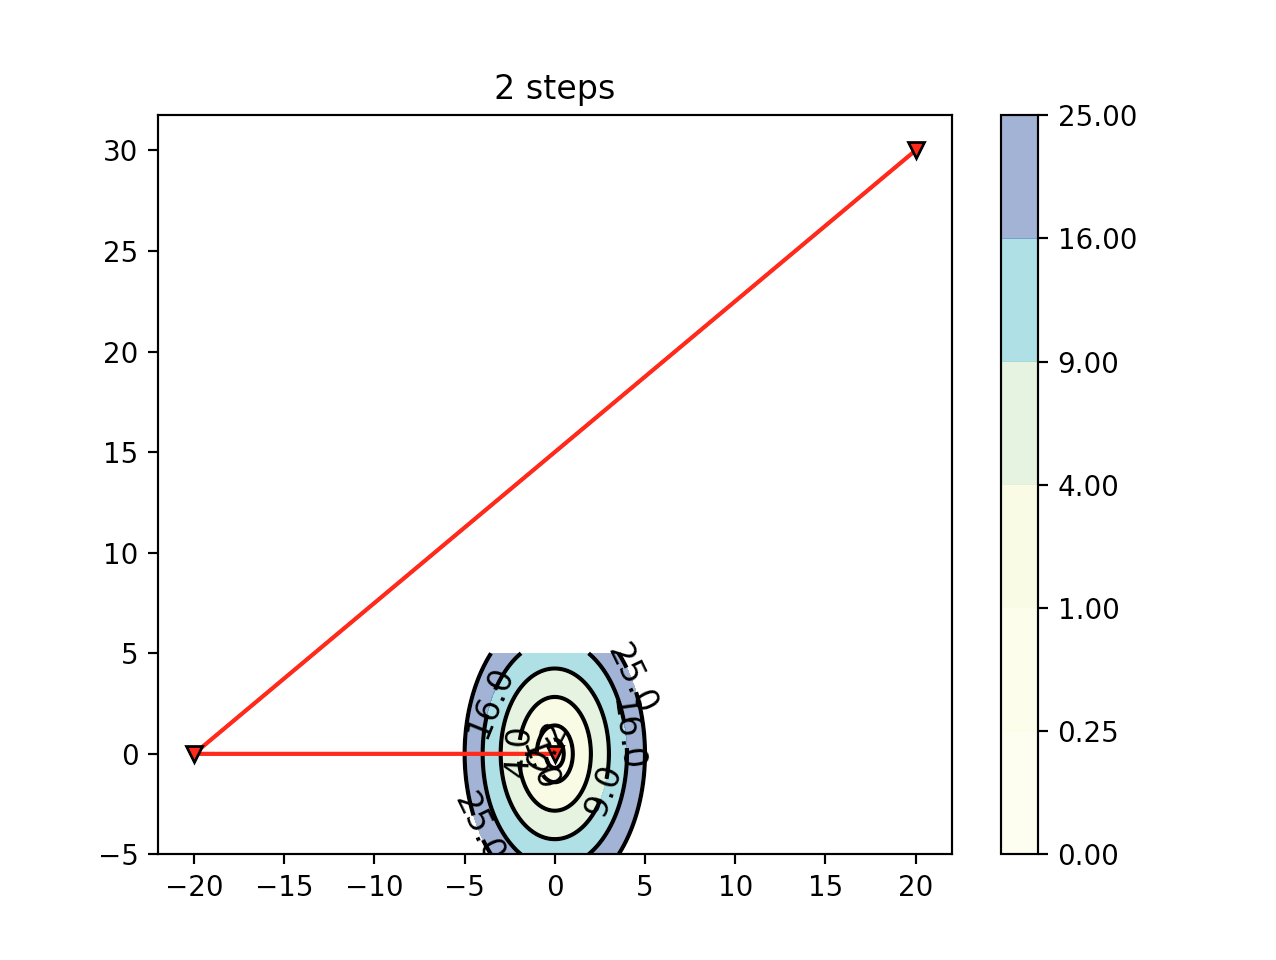
\includegraphics[width=0.49\linewidth]{12.png} \\
 a)$M_1,\ x_1$ & b)$M_1,\ x_2$\\
\end{tabular}
\end{center}

\begin{center}
\begin{tabular}{cc}
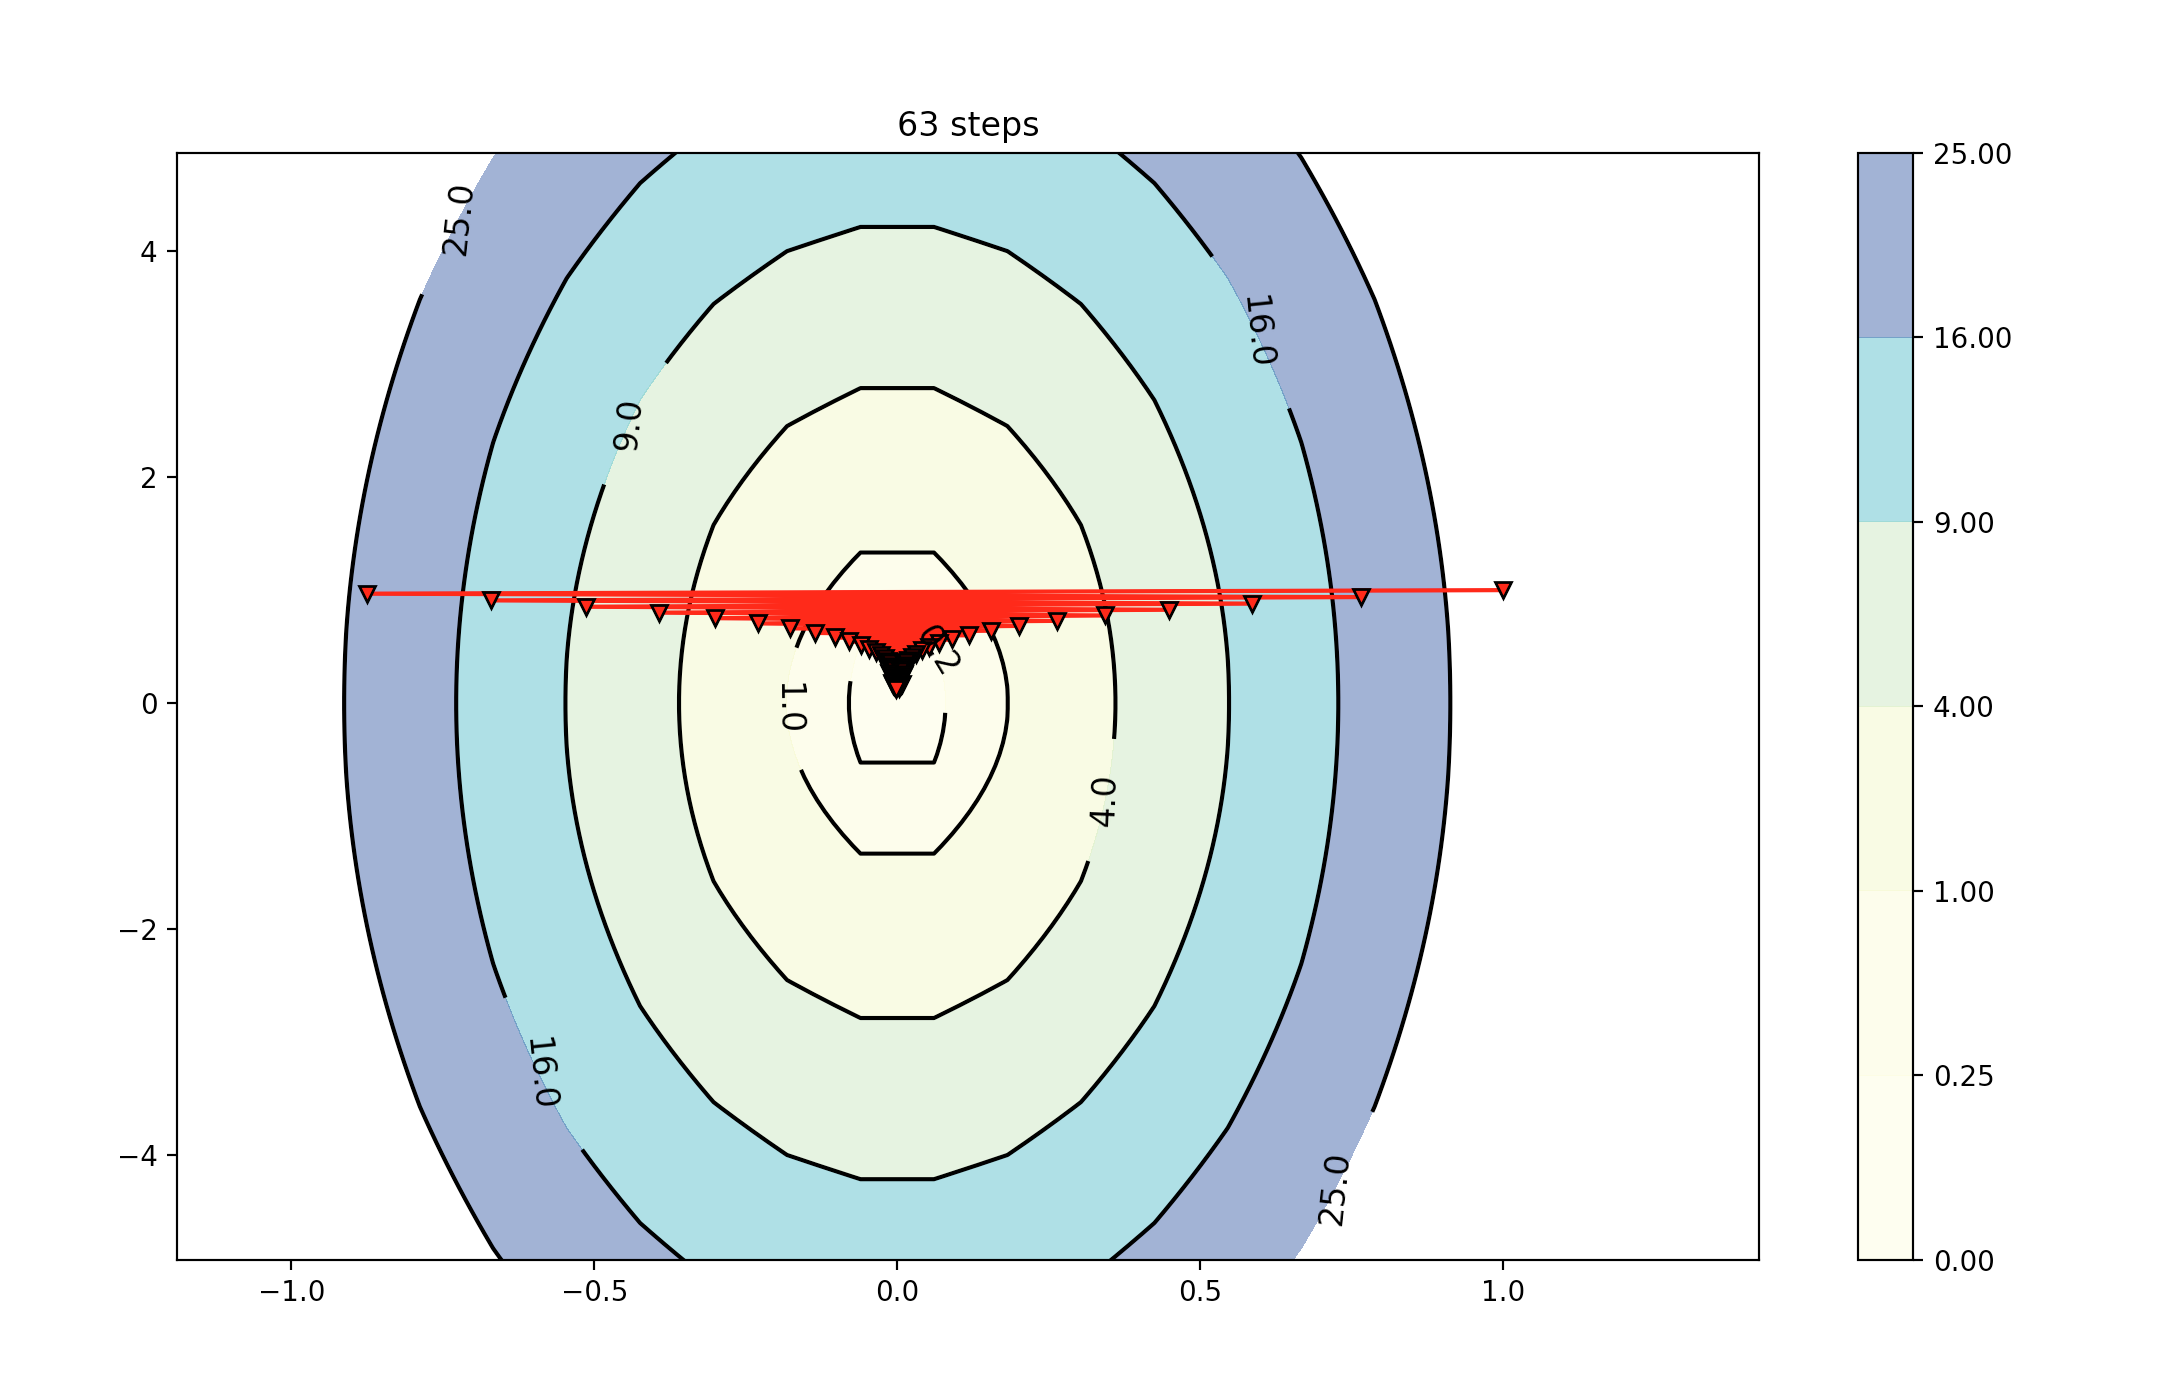
\includegraphics[width=0.49\linewidth]{13.png} &
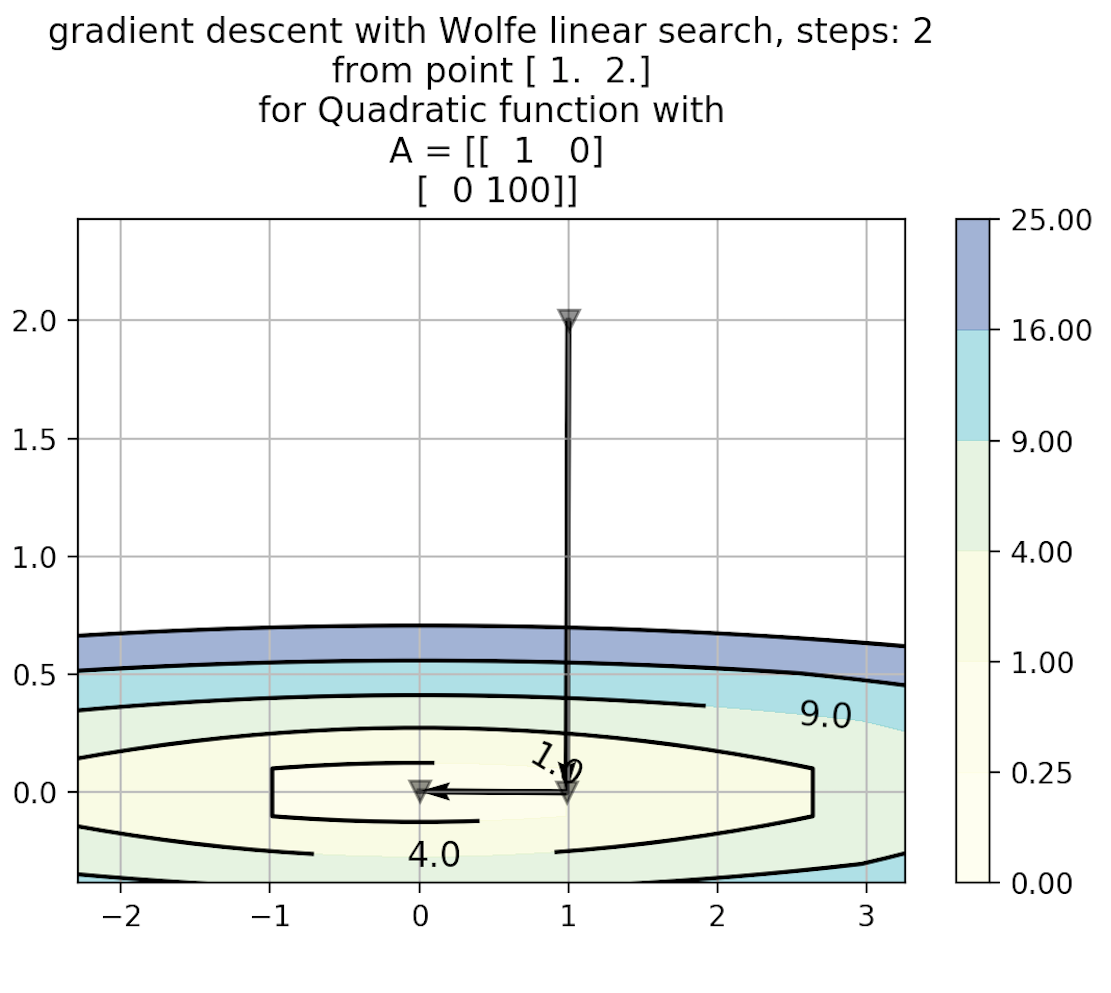
\includegraphics[width=0.49\linewidth]{14.png} \\
 a)$M_2,\ x_1$ & b)$M_2,\ x_2$\\
\end{tabular}
\end{center}


$\bullet$ Wolfe

Данный метод показал себя лучше чем все предыдущие. Отсутствует зависимость скорости сходимости от обусловленности функции и (практически) от начальной точки.

\begin{center}
\begin{tabular}{cc}
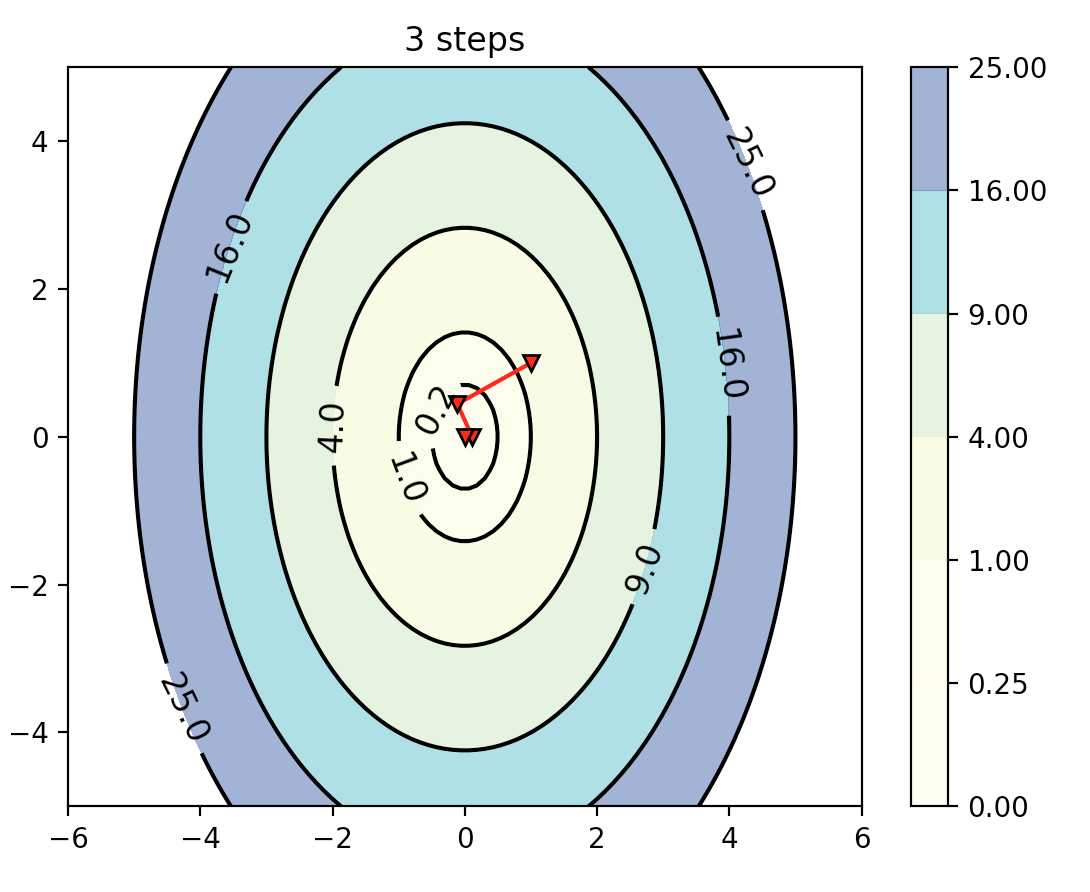
\includegraphics[width=0.49\linewidth]{19.png} &
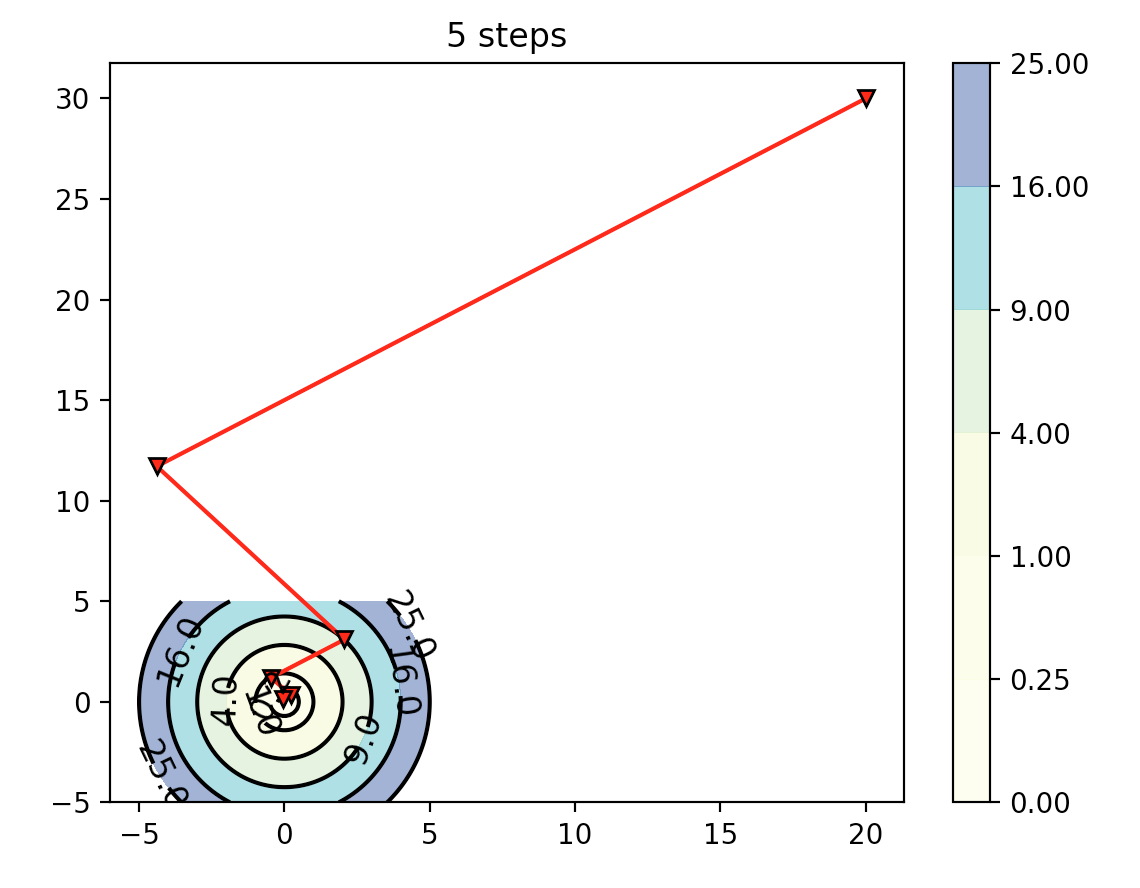
\includegraphics[width=0.49\linewidth]{110.png} \\
 a)$M_1,\ x_1$ & b)$M_1,\ x_2$\\
\end{tabular}
\end{center}

\begin{center}
\begin{tabular}{cc}
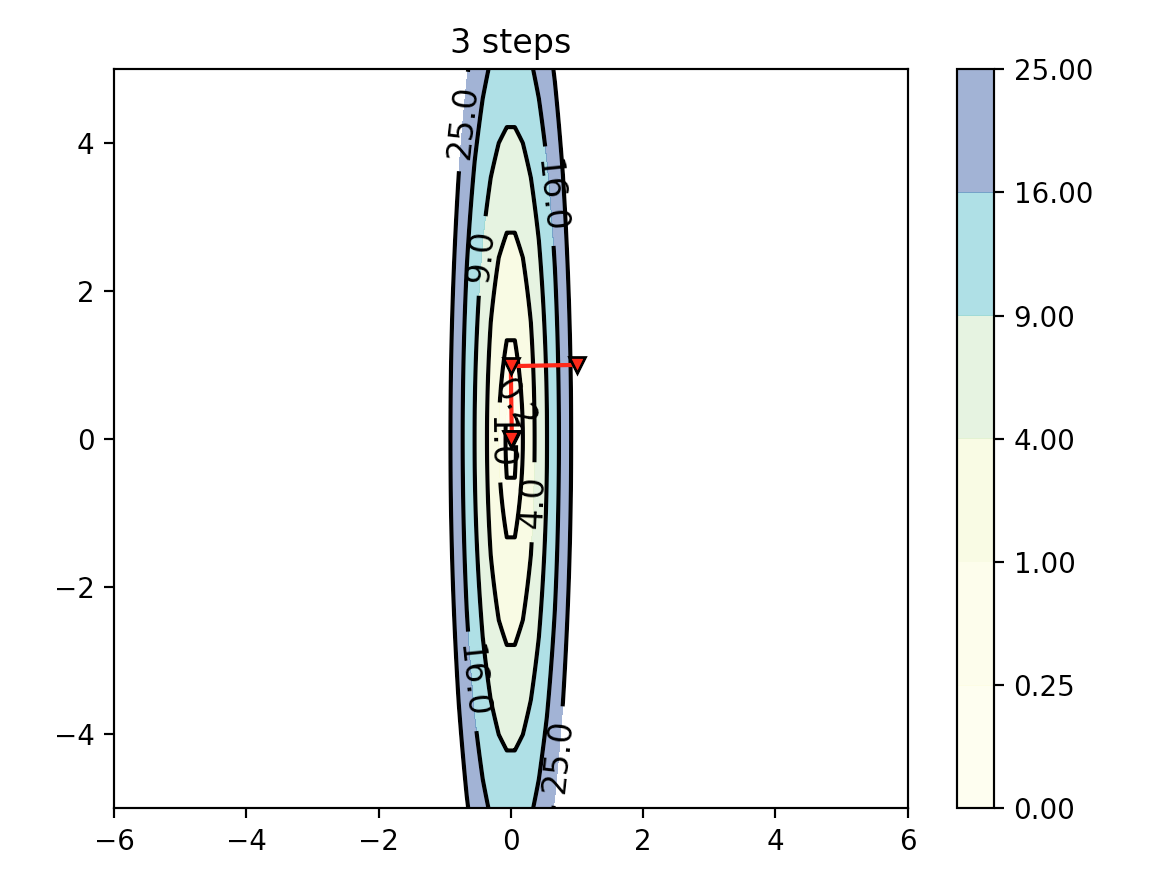
\includegraphics[width=0.49\linewidth]{111.png} &
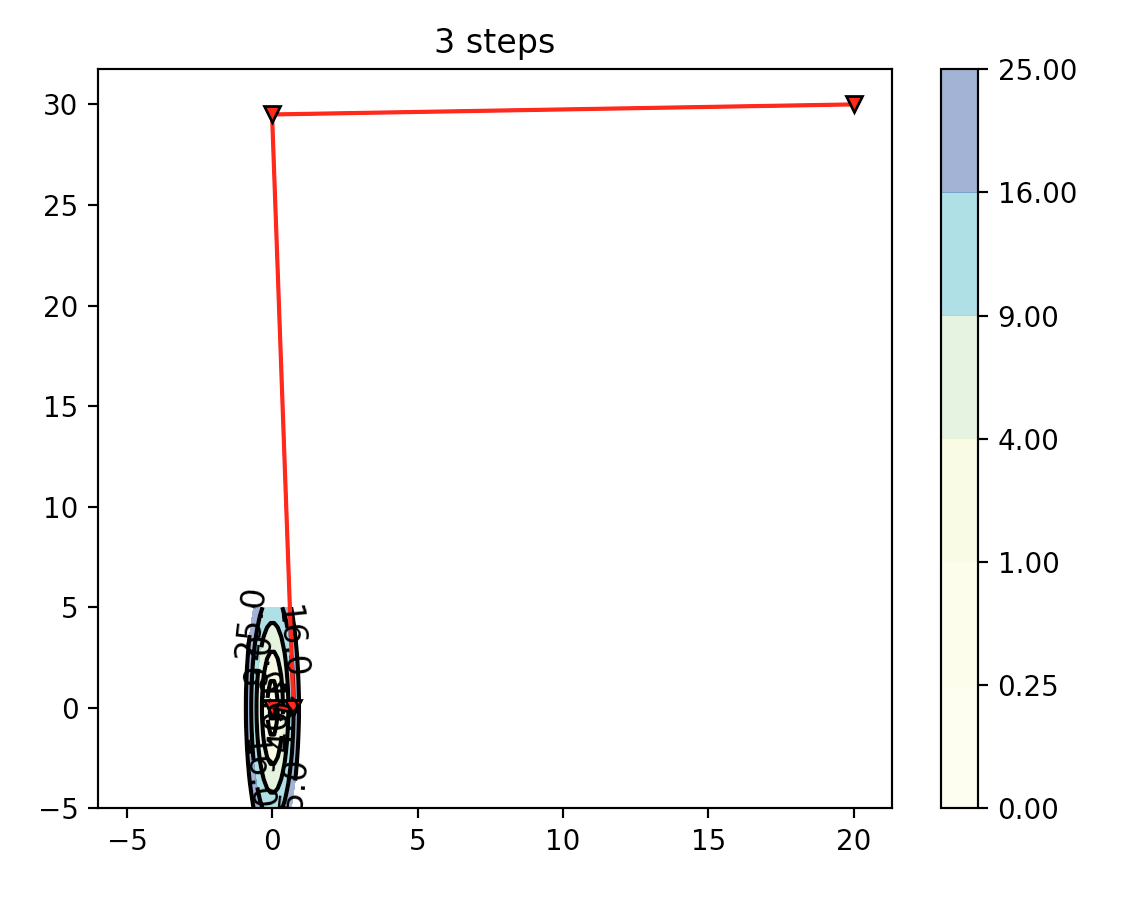
\includegraphics[width=0.49\linewidth]{112.png} \\
 a)$M_2,\ x_1$ & b)$M_2,\ x_2$\\
\end{tabular}
\end{center}

\section{Зависимость числа итераций градиентного спуска от числа обусловленности и размерности пространства.}

Для проведения данного эксперимента случайным образом были сгенерированы матрицы с различной обусловленностью из пространства различной размерности.
На полученных данных был запущен градиентный спуск.
По результатам работы градиентного спуска был построен график, по вертикальной оси отложено количество итераций совершенных алгоритмом, а по горизонтальной оси обусловленность задачи.

Из полученного графика видно что при увеличении обусловленности задачи растет количество итераций. При увеличении размерность пространства количество итераций уменьшается, причем чем больше n тем медленнее это уменьшение.

Так же можно заметить что чем больше n тем меньше разброс пунктирных линий то есть количество итераций растет стабильней.

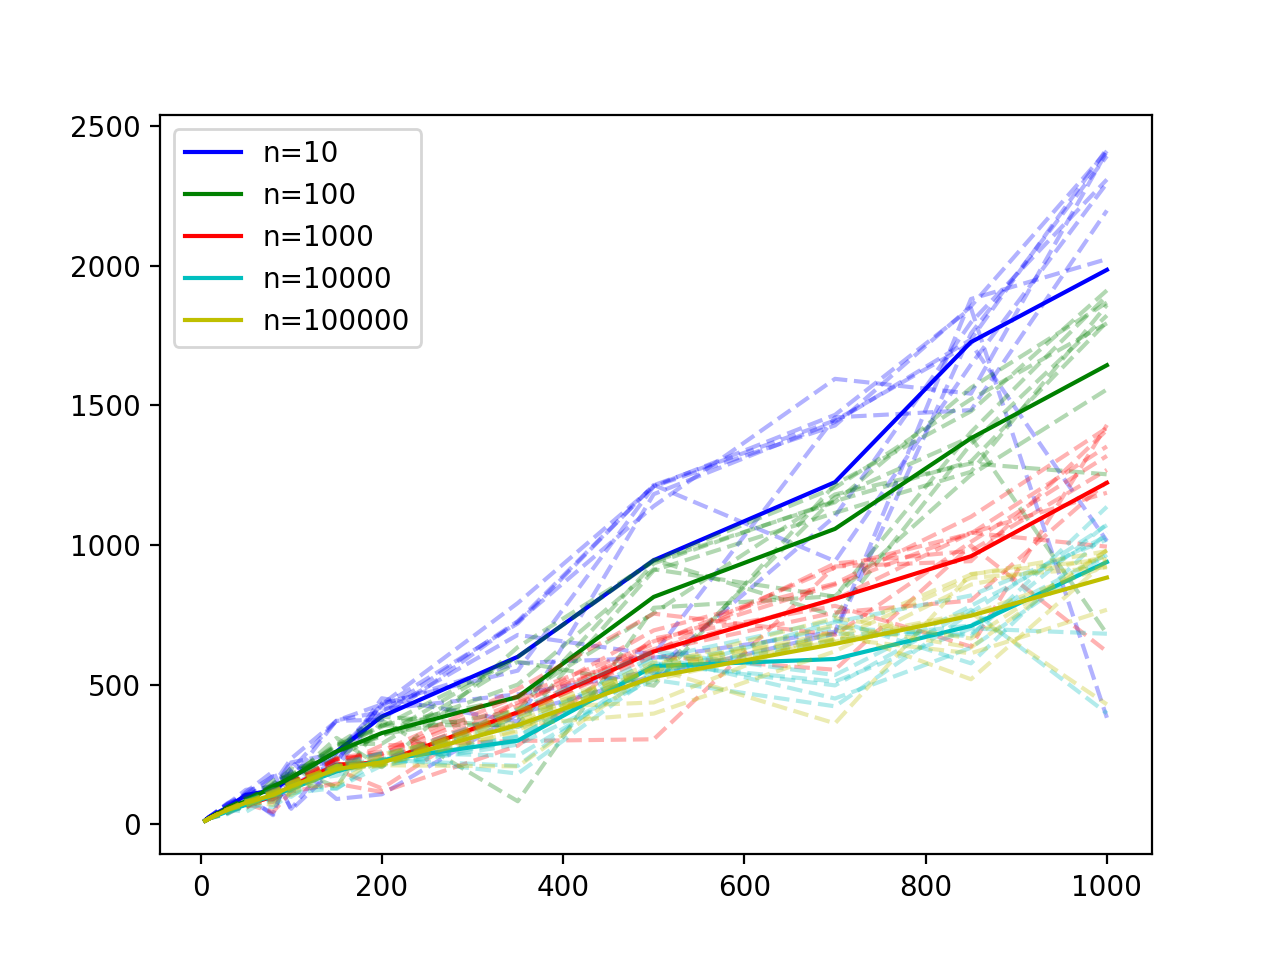
\includegraphics[width=1 \textwidth]{21.png}


\section{Сравнение методов градиентного спуска и Ньютона на реальной задаче логистической регрессии.}


Стоимость шага


На каждой итерации метода ньютона надо решить $\nabla^2 f(x_k)d_k = - \nabla f(x_k)$, данная операция при использовании разложения Холецкого занимает $O(n^3)$ и вычисление гессиана занимает $O(n^2*k)$ получаем $O(n^2*k + n^3)$
Для граиентного спуска $O(n * m)$.

Память

Метод ньютона использует $O(n^2)$ памяти, а градиентный спуск $O(n)$



В данном данном эксперименте сравнивается работа градиентного спуска с методом ньютона. Работа данных методов рассматривается на трех датасетах.


w8a

Метод Ньютона сошелся гораздо быстрее чем градиентный спуск, это произошло из за того что размер данной выборки достаточно мал и шаги метода Ньютона более агрессивны, хотя это медленнее с точки зрения вычислений.

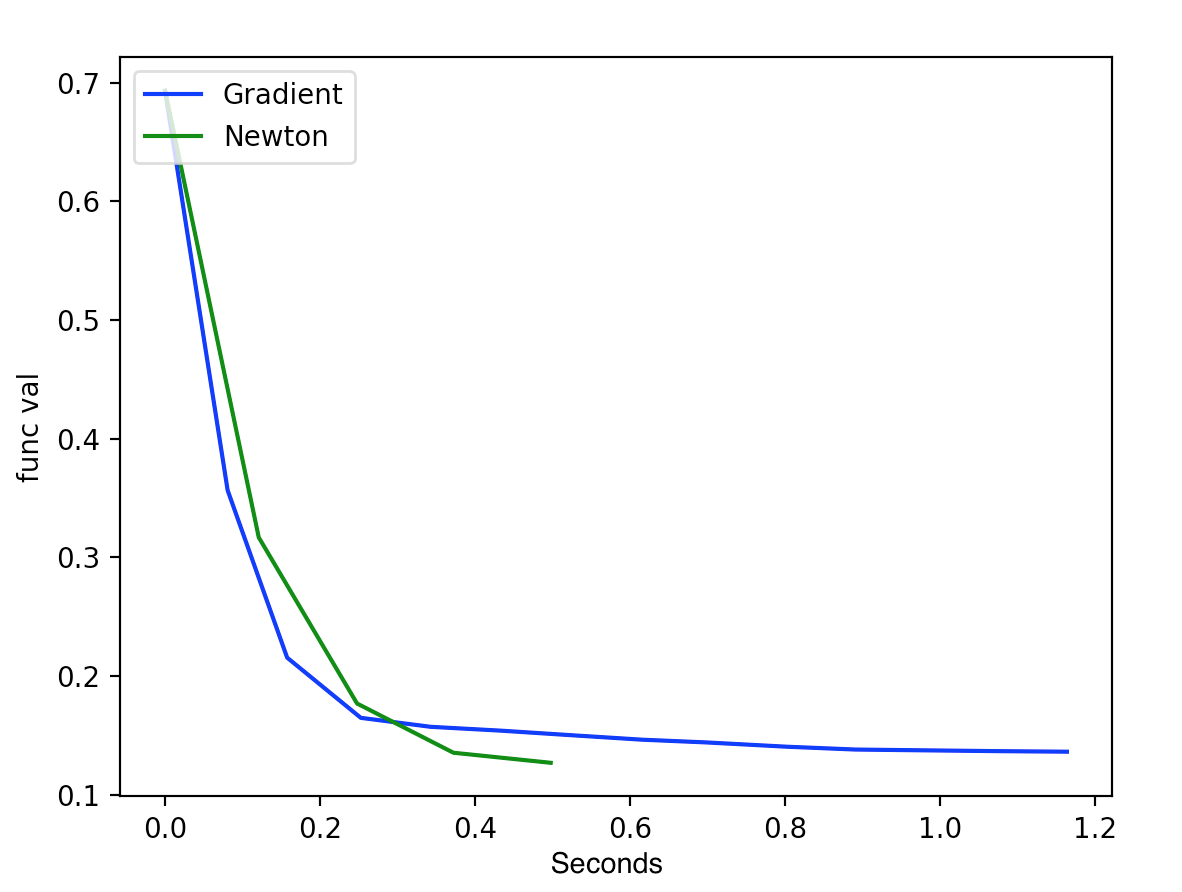
\includegraphics[width=0.6 \textwidth]{31.png}
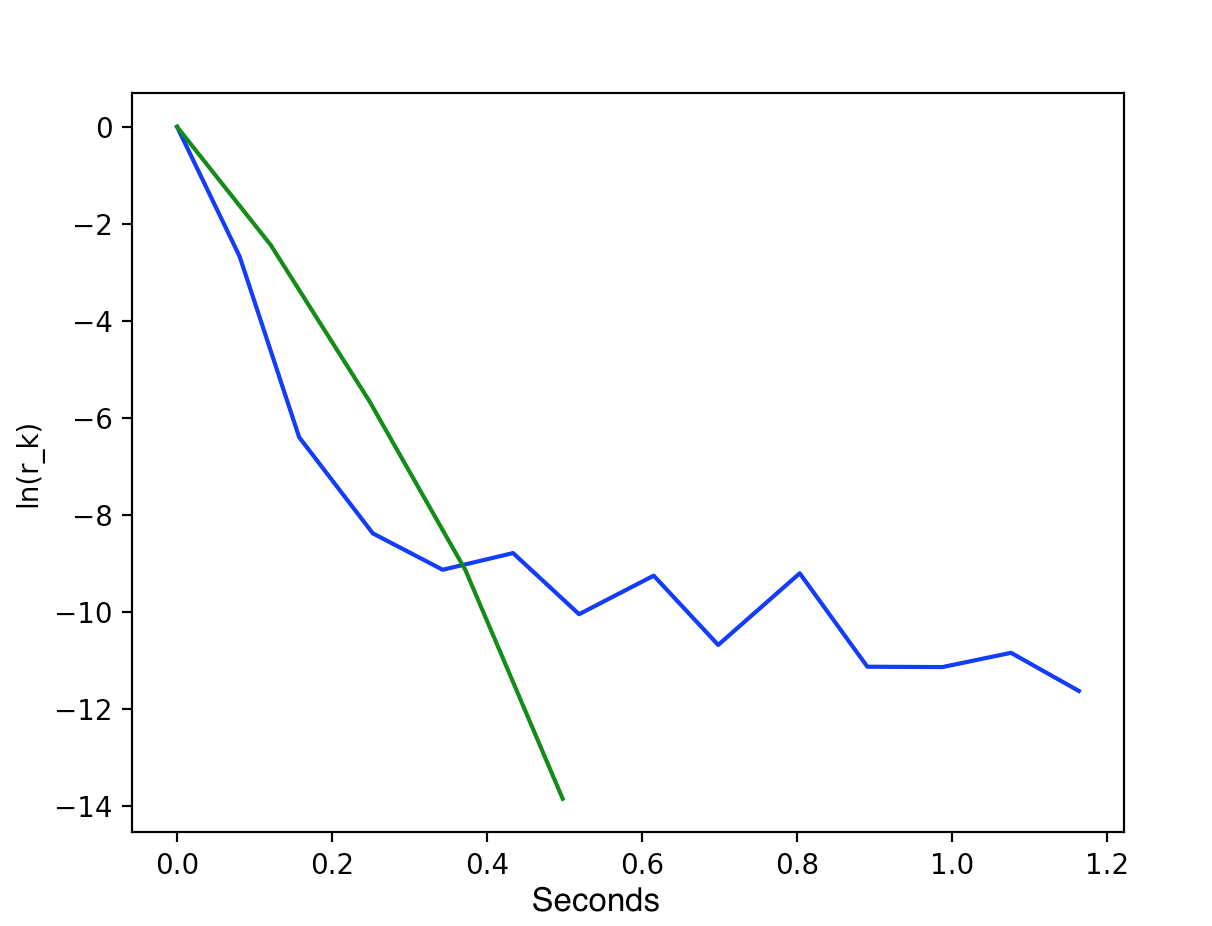
\includegraphics[width=0.6 \textwidth]{32.png}

gisette-scale

Результаты данного эксперименты отличаются от предыдущего. Данный датасет имел не так много объектов но при этом они были большого размера. Таким образом, метод Ньютона работал очень долго, и даже не смотря на то что он делает более "верные" шаги, время, которое требуется, чтобы сделать это слишком велико.

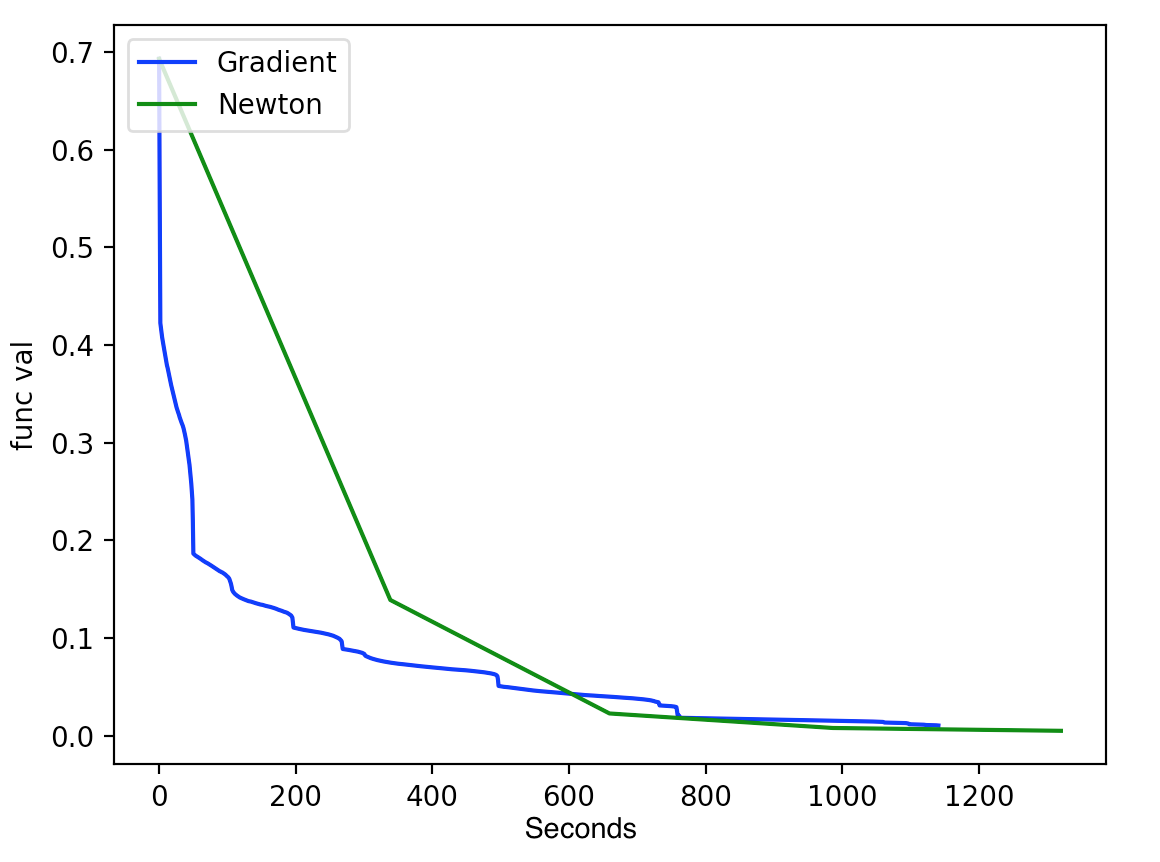
\includegraphics[width=0.6 \textwidth]{33.png}
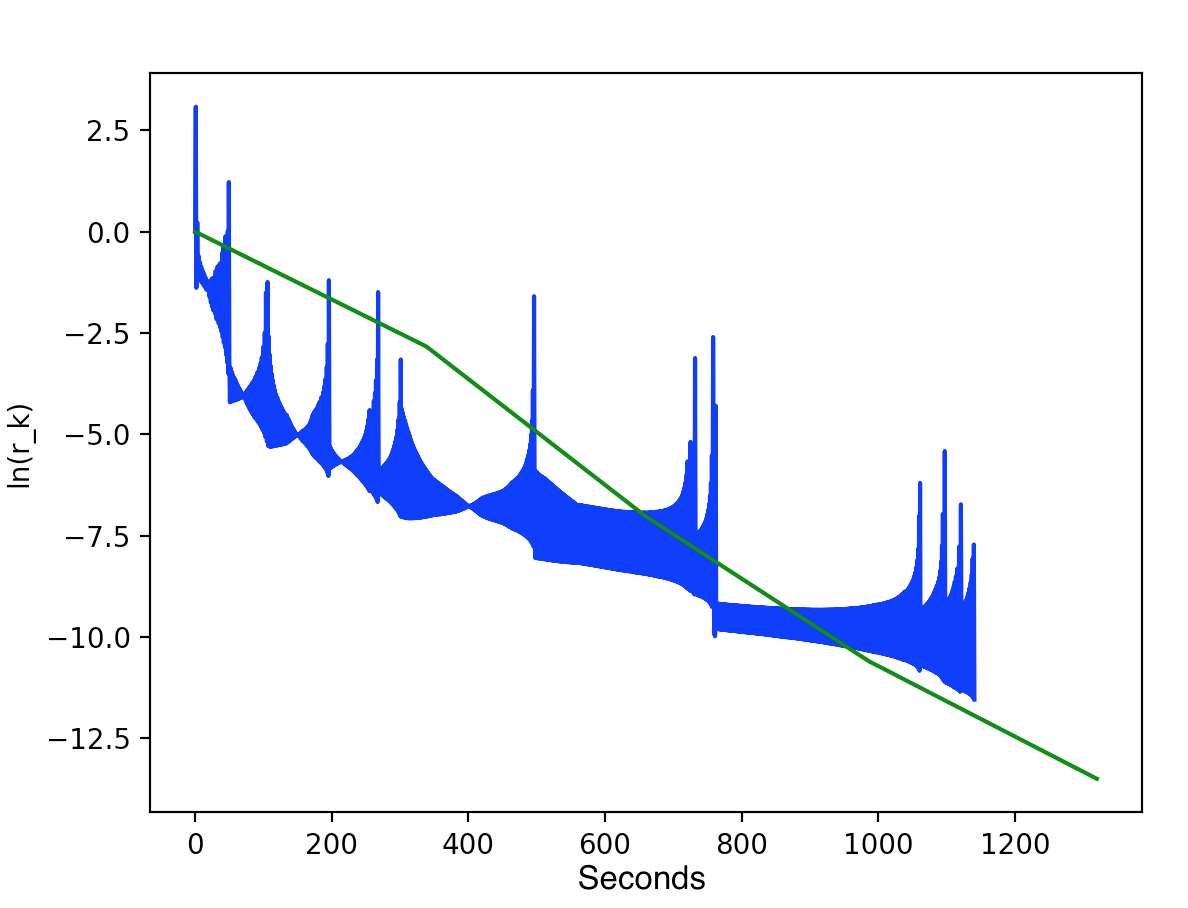
\includegraphics[width=0.6 \textwidth]{34.png}

real-sim

На данной выборке метод ньютона показал себя так же плохо, он работал во много раз дольше градиентного спуска, который, в свою очередь, показал очень хорошие результаты сойдясь чуть ли не линейно.

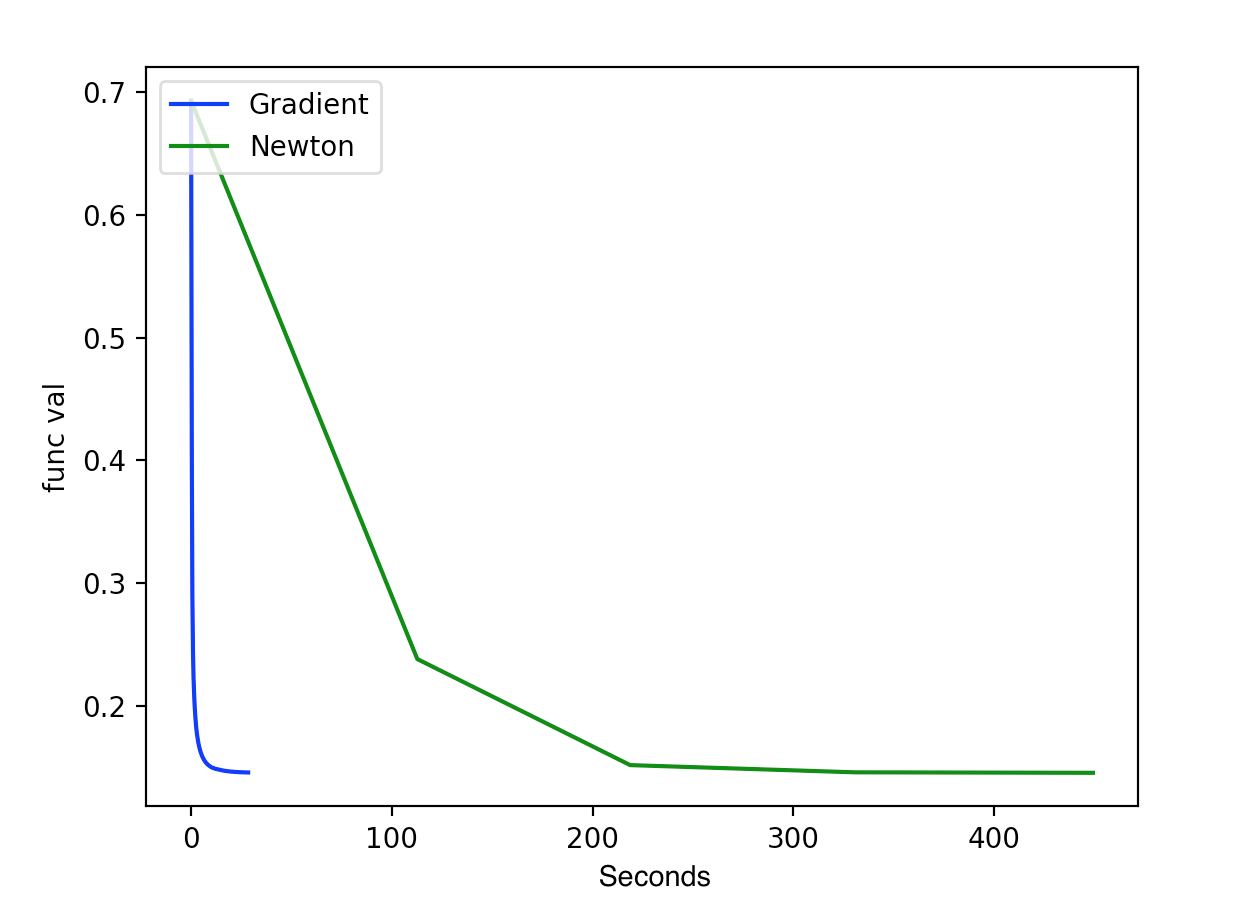
\includegraphics[width=0.6 \textwidth]{35.png}
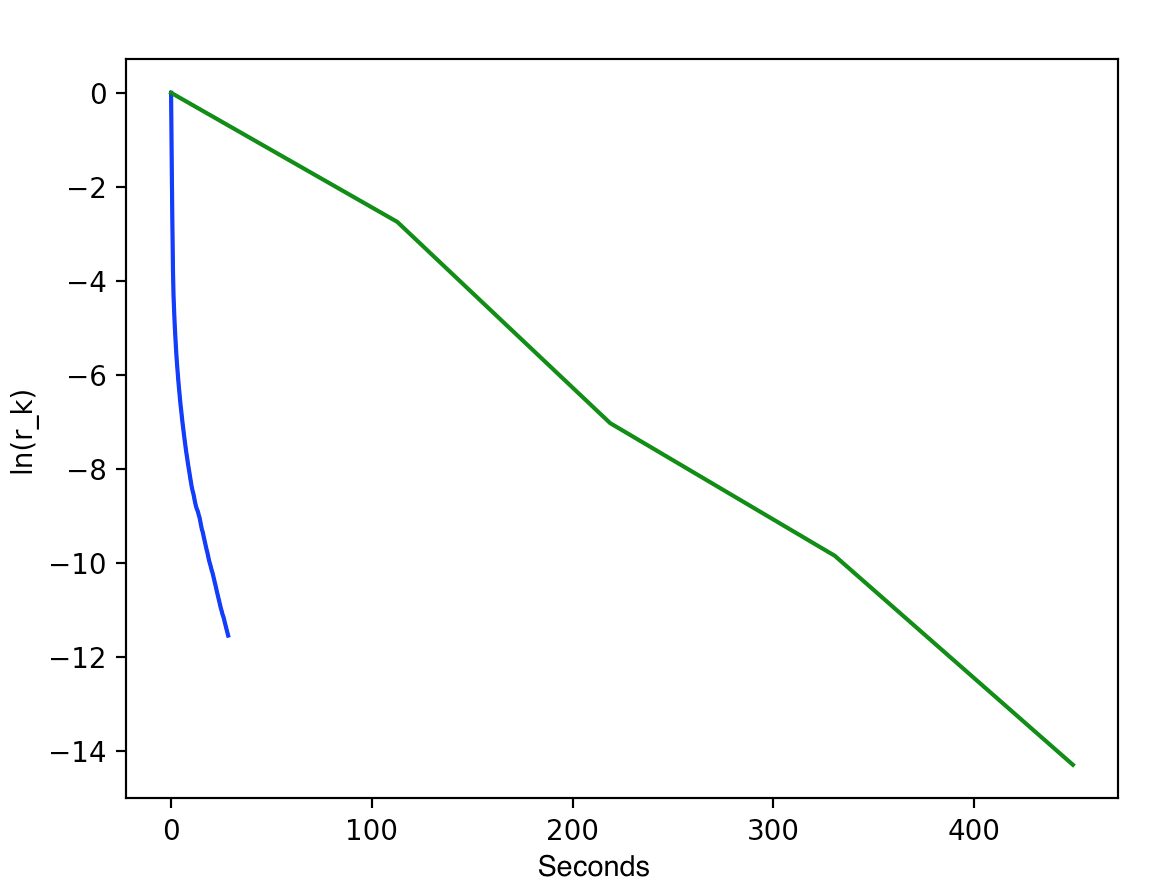
\includegraphics[width=0.6 \textwidth]{36.png}


Данный эксперимент показал как плох метод ньютона на объектах из пространства с большой размерностью. Но в пространстве объектов с малой размерностью он работает гораздо быстрее чем градиентный спуск.


\section{Оптимизация вычислений в градиентном спуске.}

Траектории обоих методов на первом графике совпадают поскольку оптимизированный оракул не отличается от обычного в плане формул использованных для вычисления градиента или значения функции. Он просто умеет быстрее посчитать значения данных функций.

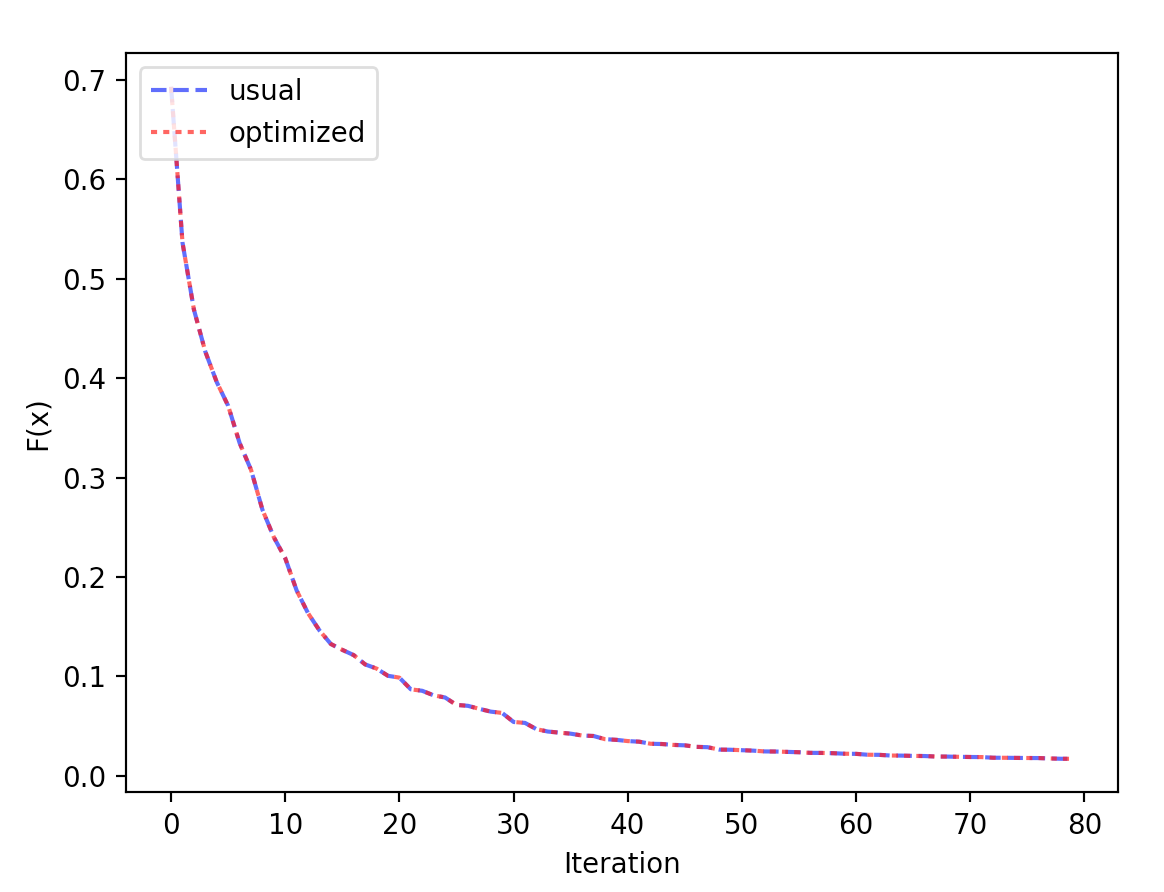
\includegraphics[width=0.6 \textwidth]{41.png}

Для данного эксперимента был реализован оптимизированный оракул, который кеширует некоторые результаты сложных операций такие как матричные умножения.

Длее был проведено сравнение работы обычного оракула и оптимизированного с помощью градиентного спуска на случайно сгенерированных данных(m, n = 10000, 8000)

Из данных графиков видно что оптимизированный оракул действительно работает гораздо быстрее чем обычный.


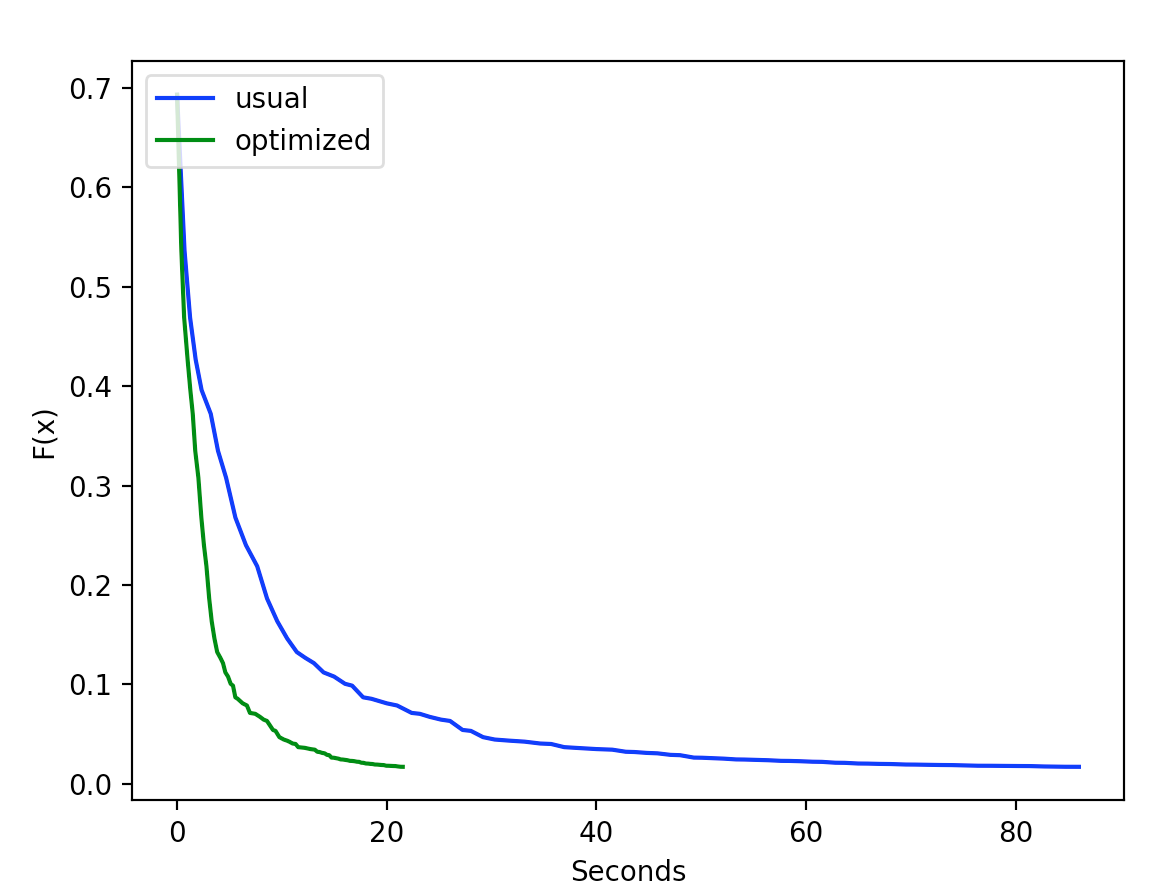
\includegraphics[width=0.6 \textwidth]{42.png}
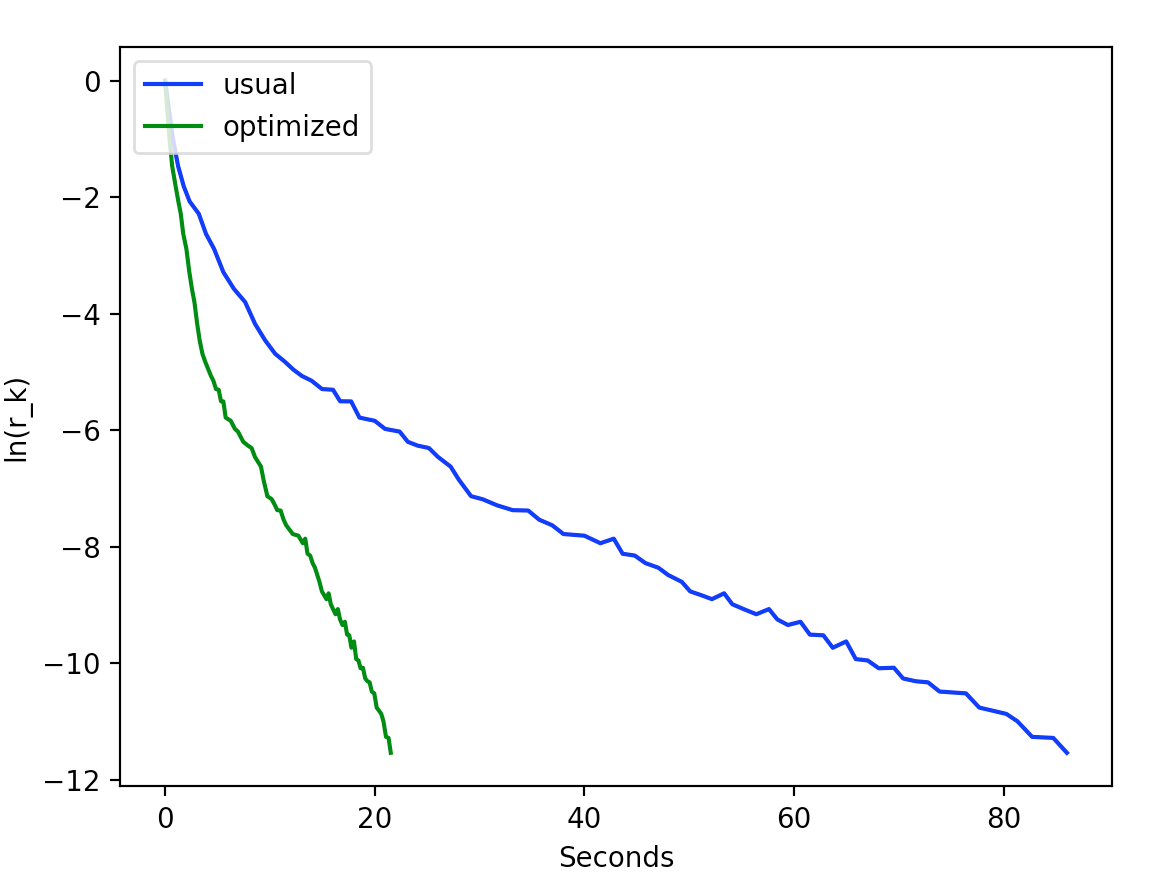
\includegraphics[width=0.6 \textwidth]{43.png}


\section{Стратегия выбора длины шага в градиентном спуске}
Для данного теста были сгенерированны случайные данные, далее на них были запущен градиент с различными стратегиями подбора шага.

Между данными стратегиями нет большой разницы, только Wolfe на левом графике ведет себя более стабильно. Сходятся данные стратегии достаточно хорошо.

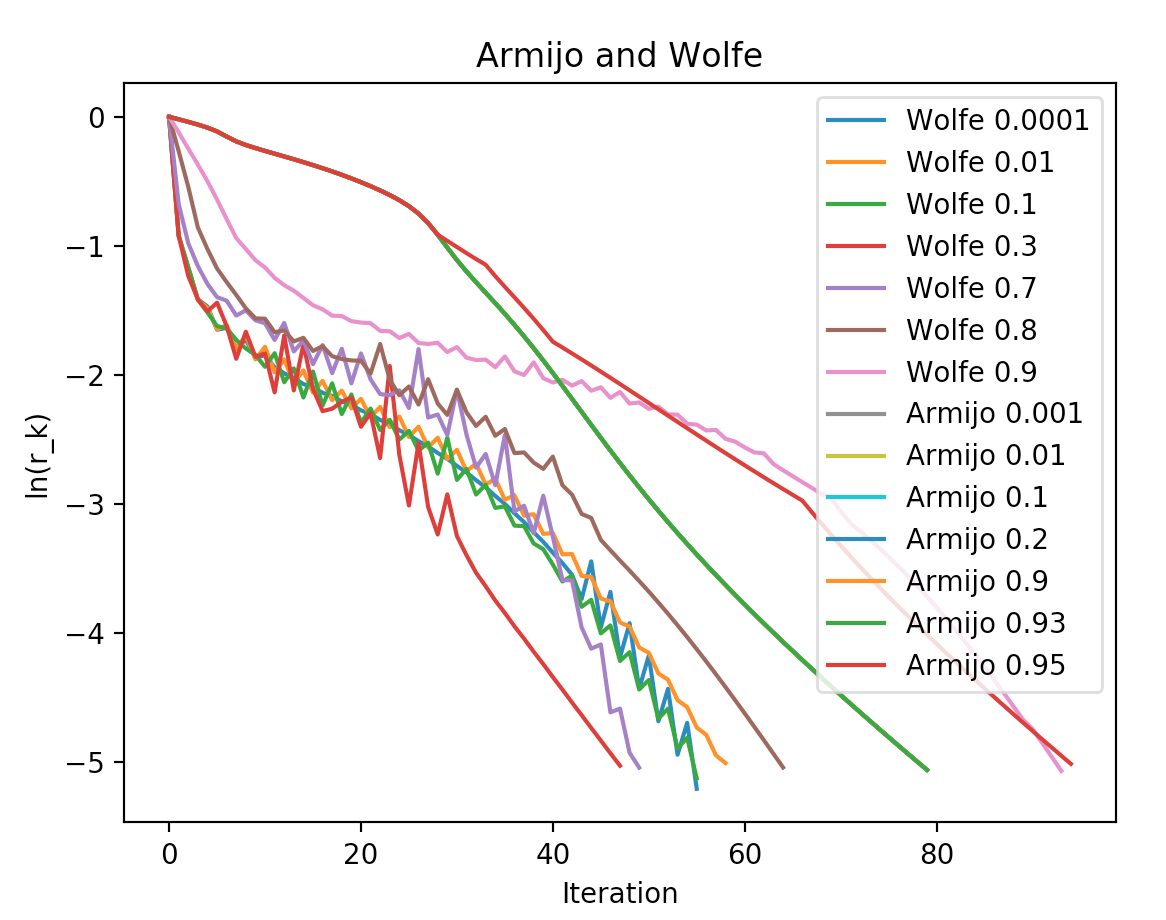
\includegraphics[width=0.6 \textwidth]{51.png}
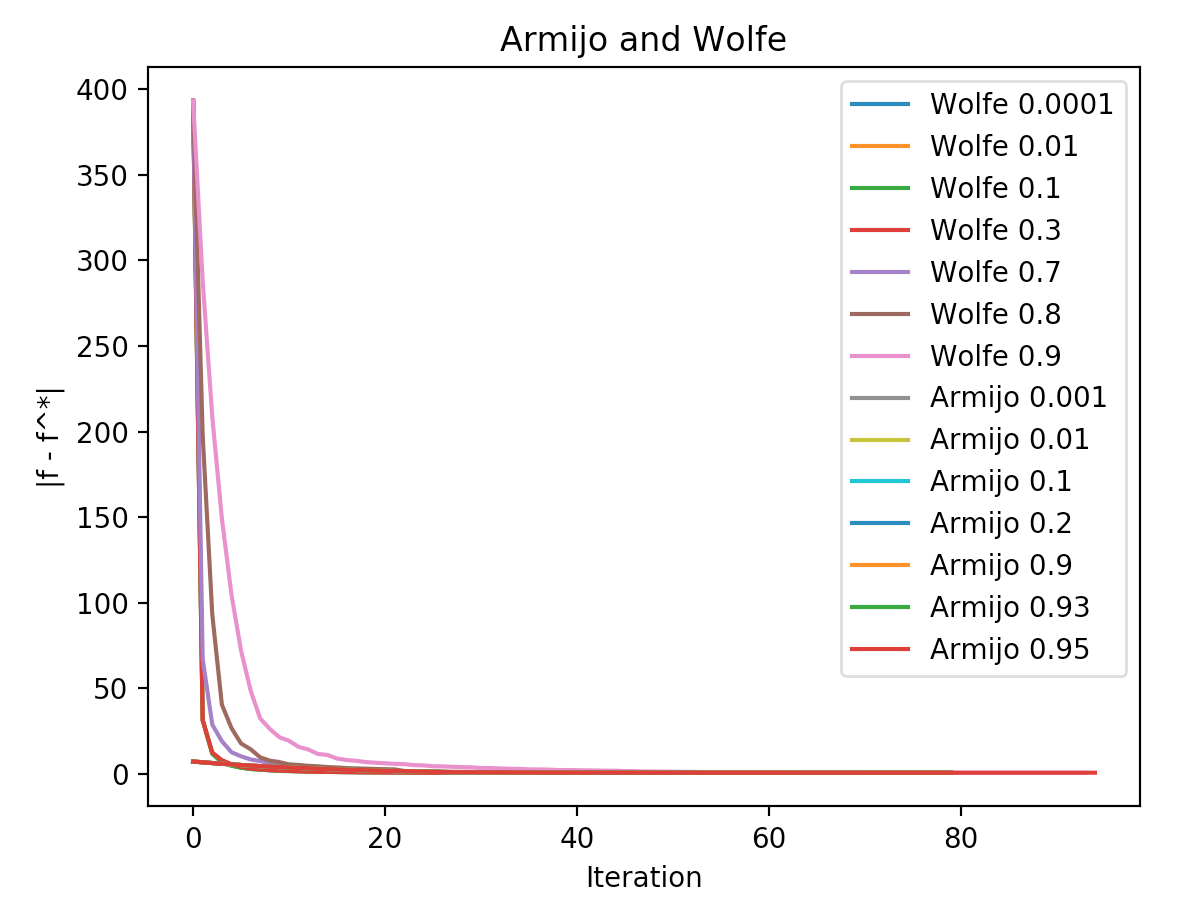
\includegraphics[width=0.6 \textwidth]{52.png}

Данная стретегия показывает себя не очень хорошо, заметна явная зависимость от выбора параметра 'c', причем если его выбрать неудачно то можно вообще не сойтись.


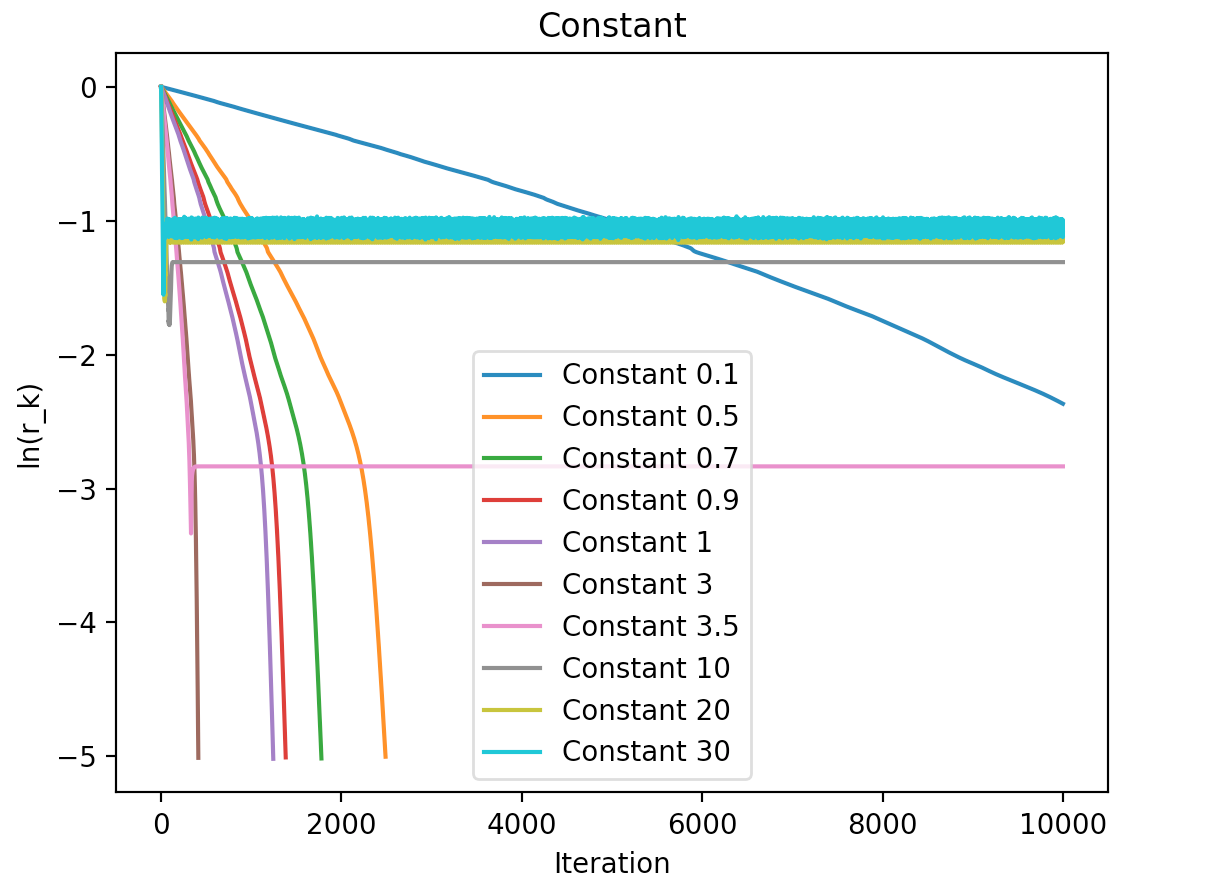
\includegraphics[width=0.6 \textwidth]{53.png}
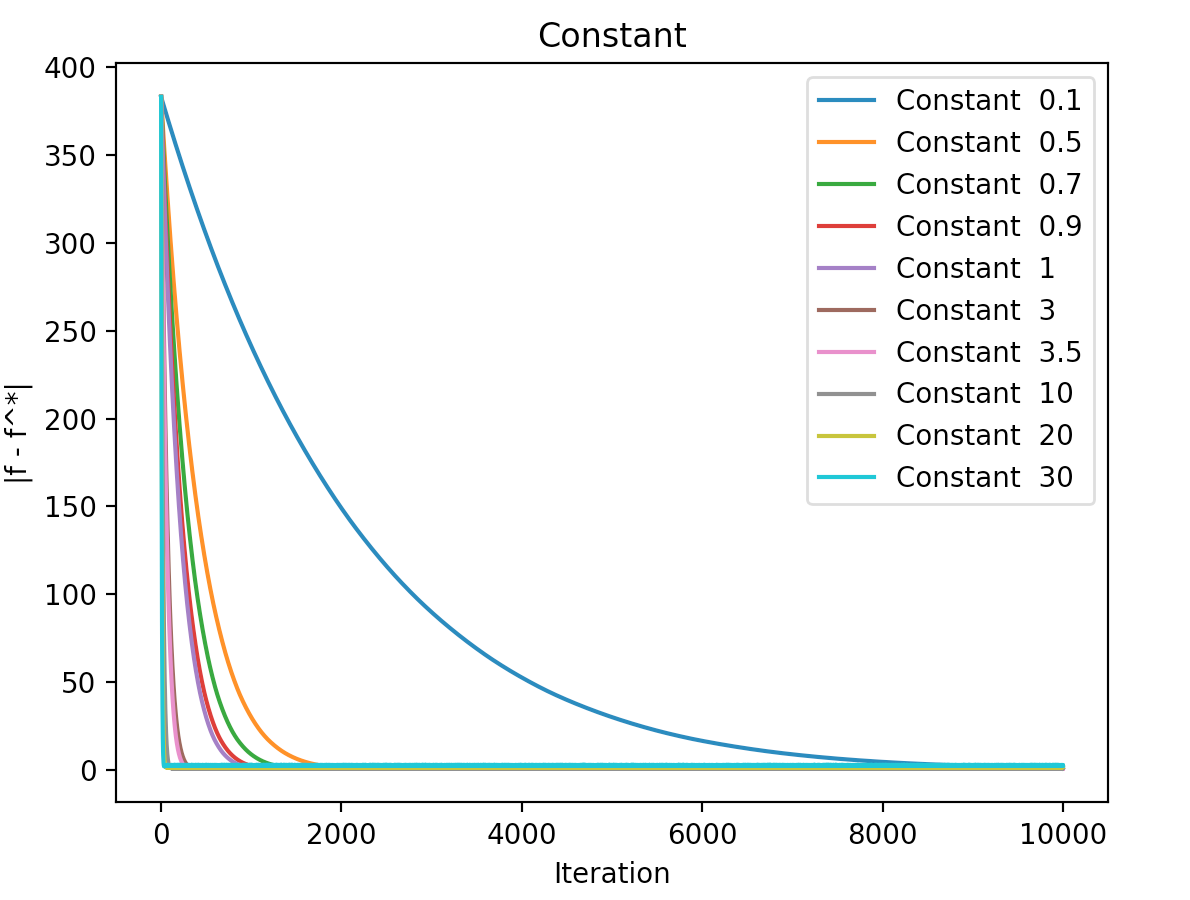
\includegraphics[width=0.6 \textwidth]{54.png}

\section{Стратегия выбора длины шага в методе ньютона}

Про данные стратегии выводы такие же как и в предыдущем эксперименте.

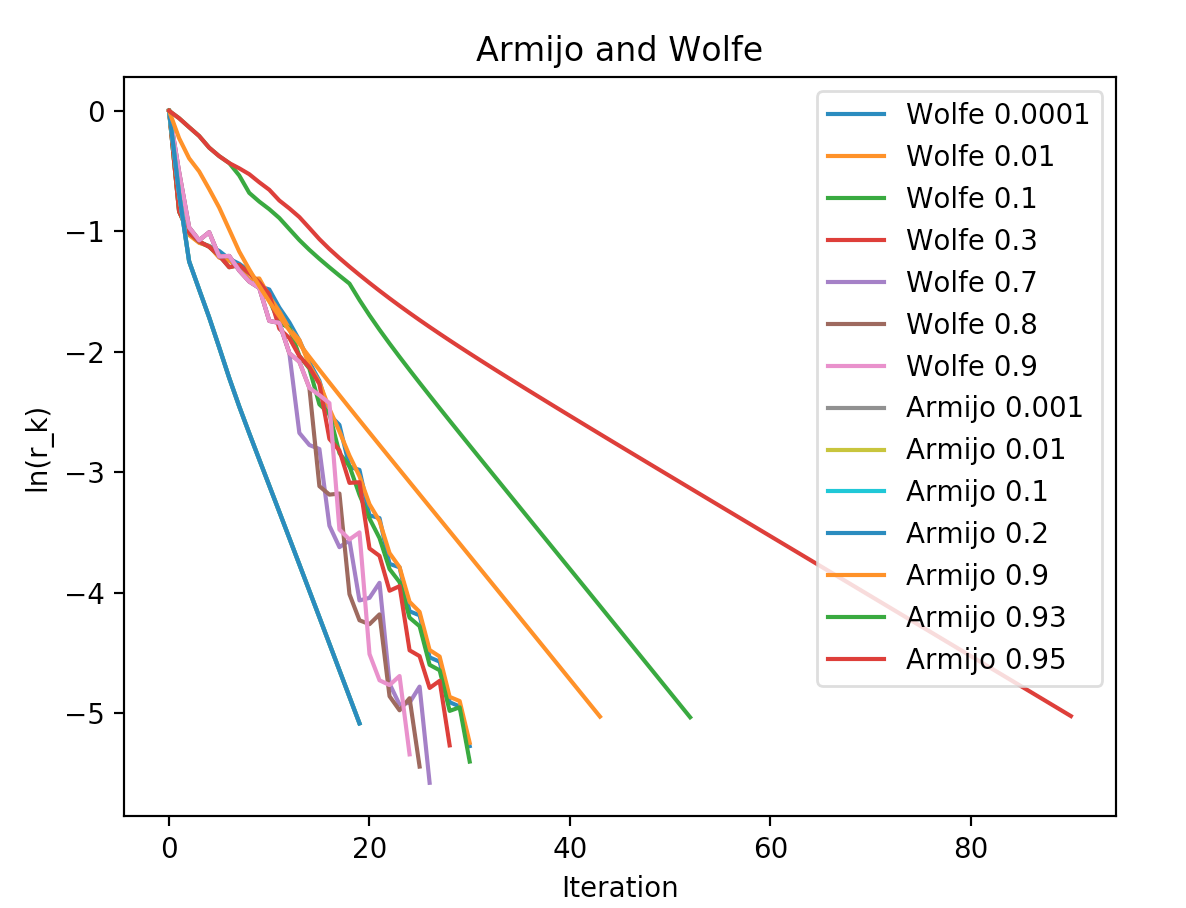
\includegraphics[width=0.6 \textwidth]{61.png}
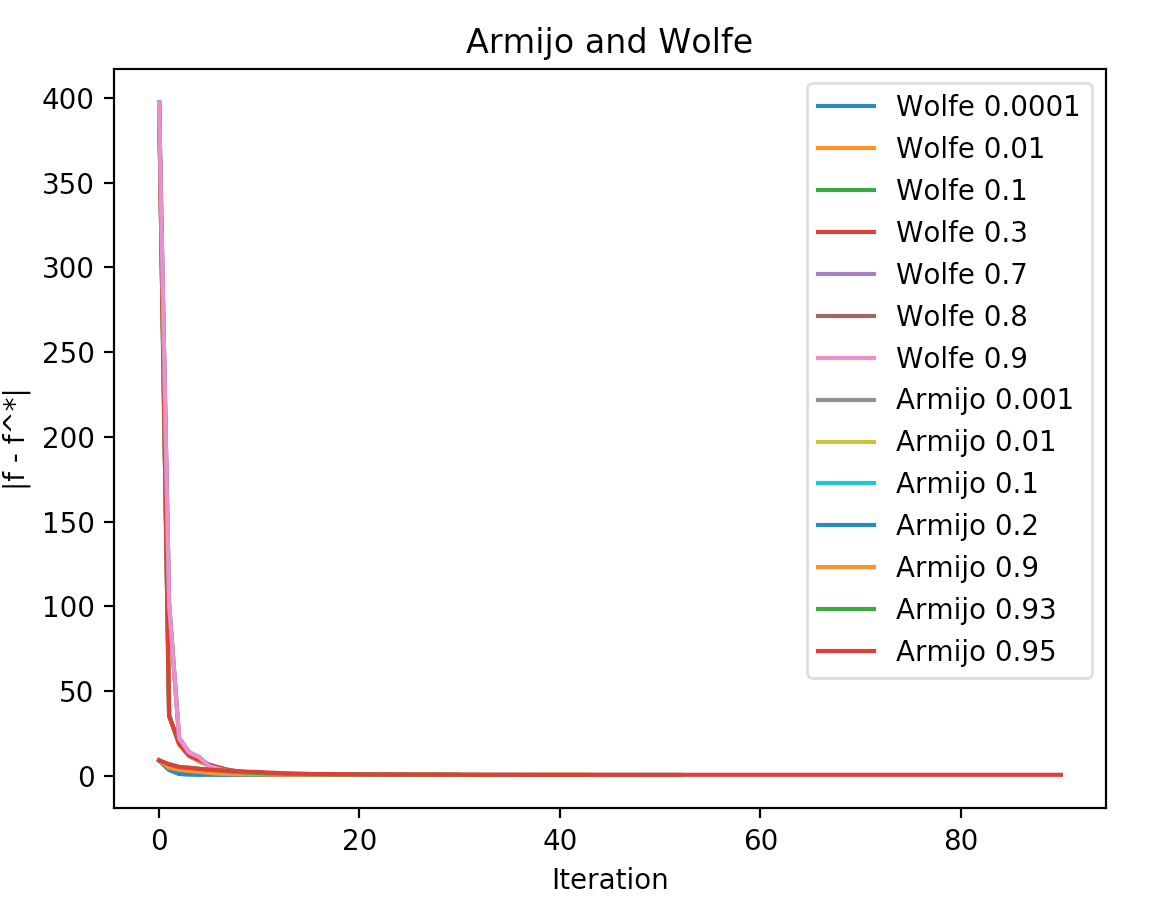
\includegraphics[width=0.6 \textwidth]{62.png}

При c > 1 видно что алгоритм не сходится(расходится). При некоторых маленьких 'c' метод сходится нормально, но при некоторых может никогда не сойтись.

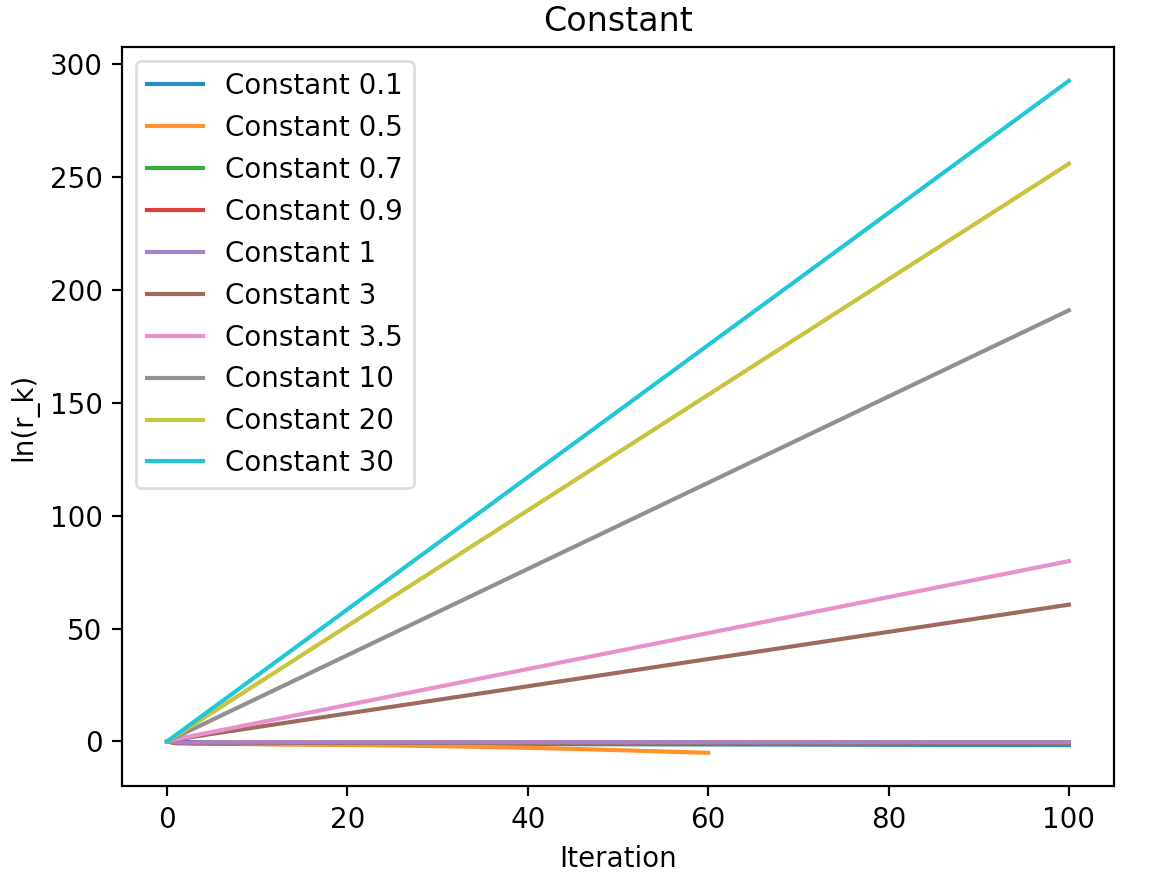
\includegraphics[width=0.6 \textwidth]{63.png}
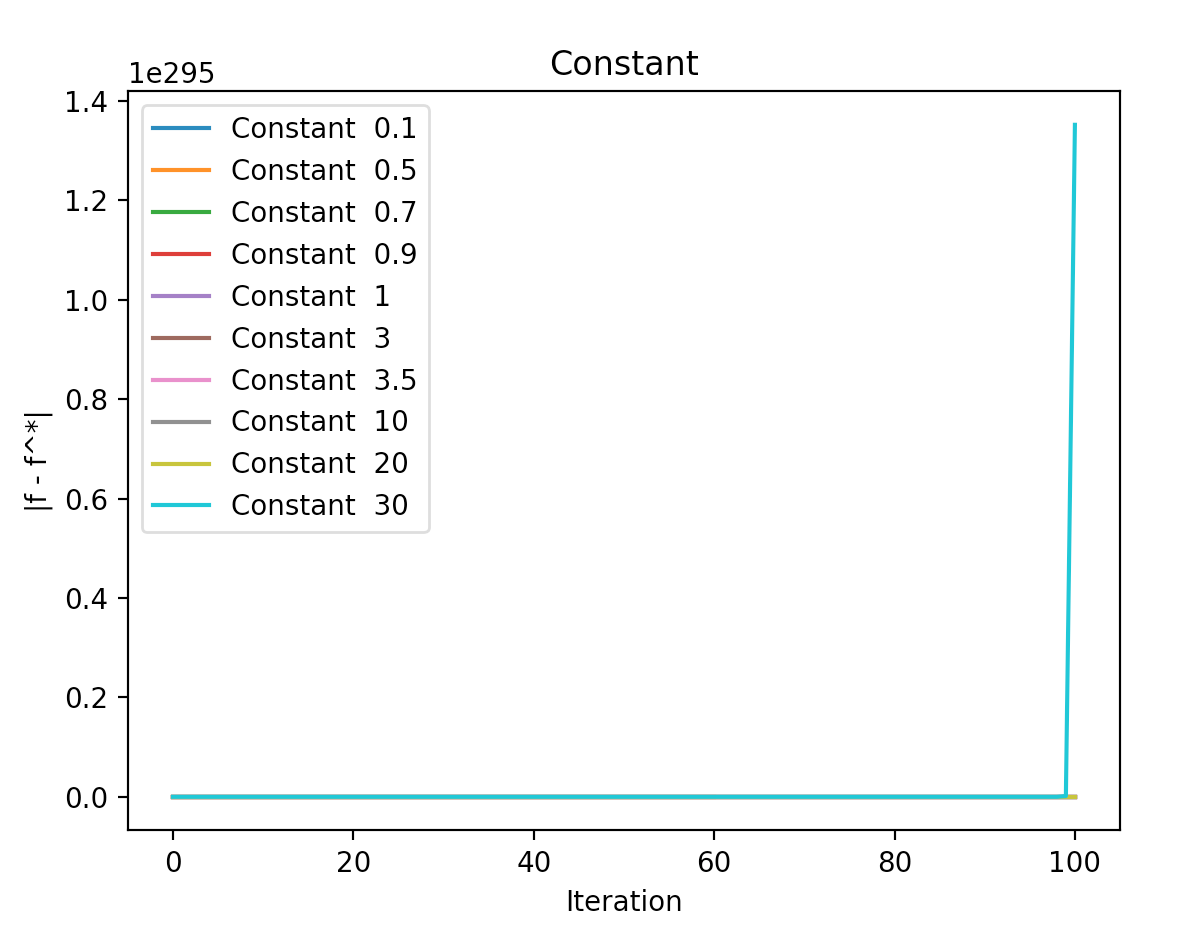
\includegraphics[width=0.6 \textwidth]{64.png}
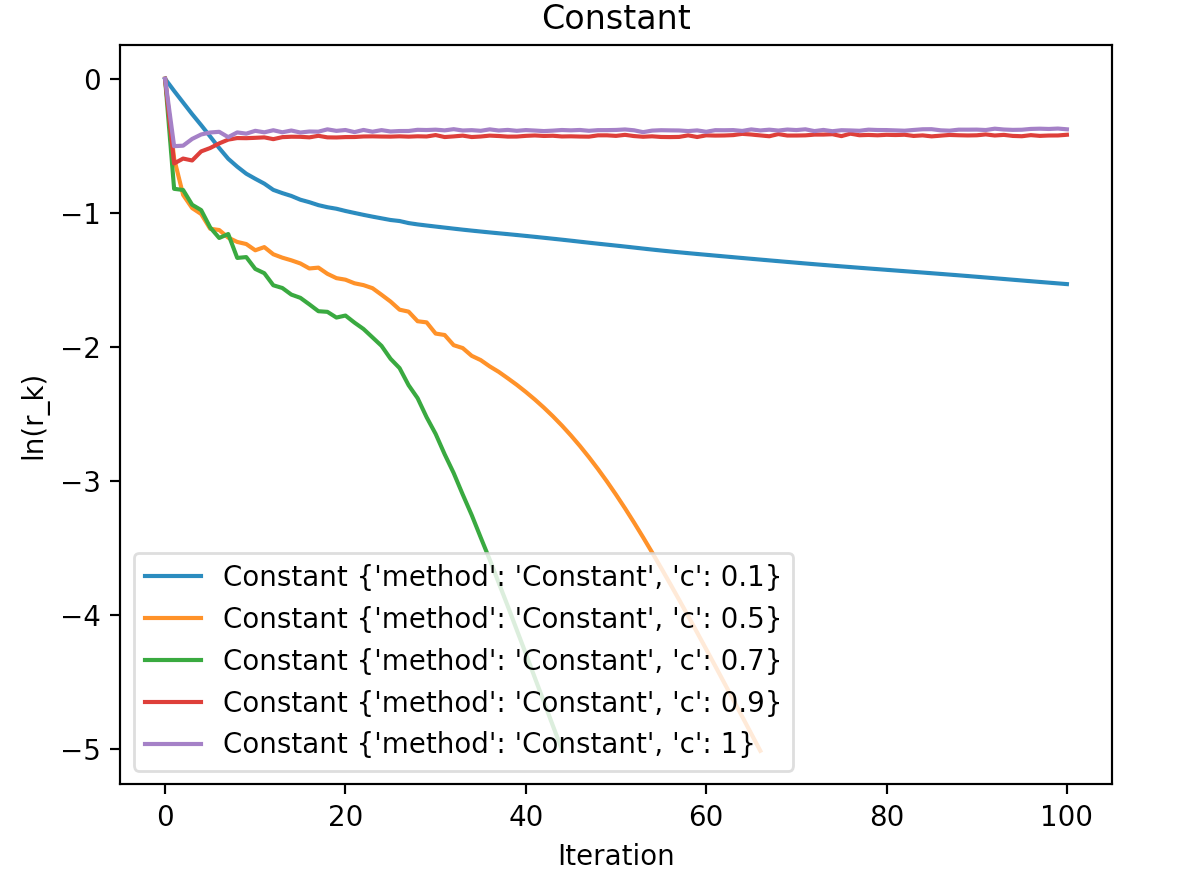
\includegraphics[width=0.6 \textwidth]{65.png}
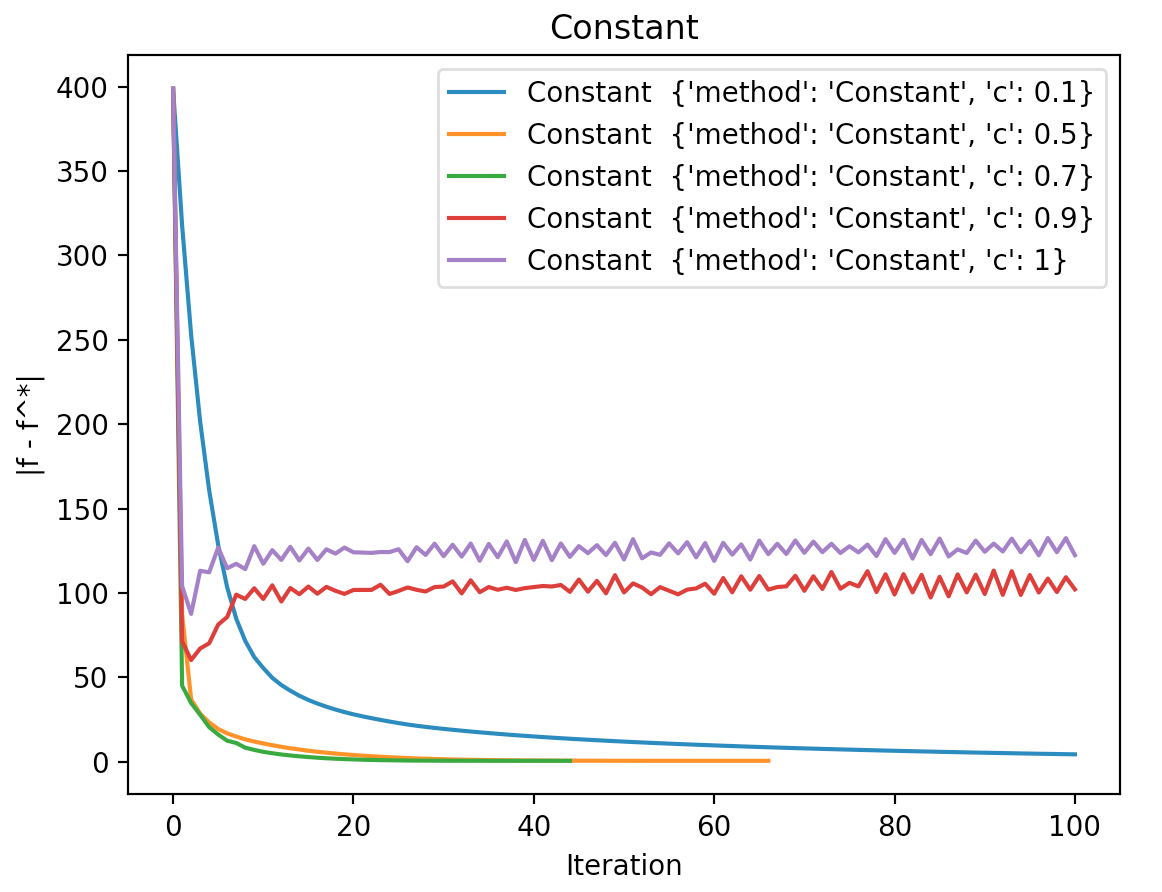
\includegraphics[width=0.6 \textwidth]{66.png}


\end{document}
